%----------------------------------------------------------
% SPIT black book. Compile with pdflatex (Overleaf default).
% Names: edit details.tex. Chapters were first generated from paper/Thesis_draft.docx by
% training/scripts/build_black_book.py and then edited directly. Do NOT re-run that script:
% it would overwrite these edits.
%----------------------------------------------------------
\documentclass[12pt]{report}
\usepackage[T1]{fontenc}
\usepackage{graphicx}
\usepackage{longtable}
\usepackage{array}
\usepackage{booktabs}
\usepackage{amsmath}
\usepackage{xcolor}
\usepackage{cite}
\usepackage{needspace}
\usepackage{etoolbox}
\pretocmd{\section}{\needspace{10\baselineskip}}{}{}
\usepackage[a4paper,width=150mm,top=25mm,bottom=25mm]{geometry}
\usepackage[hidelinks]{hyperref}
\setlength{\LTcapwidth}{\linewidth}
% All front-matter pages read from here.
\hyphenation{Chaudhari Rajkotwala Wadhwa Sheetal Dhage Pawar}
\newcommand{\ProjectTitle}{Energy Efficiency of Quantized LLM Inference: Measurement Across Serving Stacks and Evaluation of Prompt-Complexity Routing}
% One line per student on the title page; add or remove lines as needed.
\newcommand{\StudentsTitlePage}{%
{\large \textbf{Arwa Rajkotwala (2023300178)}}\\
{\large \textbf{Yessica Sule (2023300239)}}\\
{\large \textbf{Khushi Wadhwa (2023300258)}}\\
}
\newcommand{\StudentsInline}{Ms.~Arwa~Rajkotwala, Ms.~Yessica~Sule and Ms.~Khushi~Wadhwa}
\newcommand{\StudentsSignature}{%
\textbf{1. Arwa Rajkotwala}\\
\textbf{2. Yessica Sule}\\
\textbf{3. Khushi Wadhwa}\\
}
\newcommand{\GuideName}{Prof.~Sheetal~Chaudhari}
\newcommand{\HodName}{Dr.~Sudhir~Dhage}
\newcommand{\PrincipalName}{Dr.~B.~N.~Chaudhari}
\newcommand{\ExaminerName}{Prof.~Renuka~Pawar}
\newcommand{\DegreeBranch}{Computer Engineering}
\newcommand{\ReportDate}{November 2026}

\begin{document}
\begin{titlepage}
\vspace*{0.25cm}
{\centering
\large
{\Large\textbf{\ProjectTitle}}\\
\vspace{0.75cm}
submitted in partial fulfillment of the requirement\\
for the award of the Degree of\\\vspace{1cm}
{\large\textbf{Bachelor of Technology}}\\
in \\
{\large\textbf{\DegreeBranch}}\\
\vspace{0.75cm}
by\\
\vspace{0.75cm}
\StudentsTitlePage
\vspace{0.75cm}
under the guidance of\\
\vspace{0.75cm}
{\large\textbf{\GuideName}}\\
\vspace{0.5cm}

\includegraphics[scale=0.8]{spitlogo.pdf}\\
\vspace{0.5cm}
\textbf{Department of \DegreeBranch}\\
Bharatiya Vidya Bhavan's\\
Sardar Patel Institute of Technology\\
(Autonomous Institute Affiliated to University of Mumbai)\\
Munshi Nagar, Andheri-West, Mumbai-400058\\
University of Mumbai\\
\ReportDate\par}
\end{titlepage}
\newpage

\thispagestyle{empty}
\vspace*{0.2cm}
\vspace{1cm}
\begin{center}
\large\textbf{Certificate}
\end{center}
\vspace{1cm}
This is to certify that the Project entitled ``\ProjectTitle'' has been completed to our satisfaction by \StudentsInline\ under the guidance of \GuideName\ for the award of Degree of Bachelor of Technology in \DegreeBranch\ from University of Mumbai.\par
\vspace{1cm}
\begin{center}
\textbf{Certified by}
\end{center}
\vspace{1cm}

\noindent\begin{minipage}[t]{0.48\linewidth}
\textbf{\GuideName}\\
\textbf{Project Guide}
\end{minipage}\hfill
\begin{minipage}[t]{0.48\linewidth}\raggedleft
\textbf{\HodName}\\
\textbf{Head of Department}
\end{minipage}
\vspace{1cm}

\begin{center}
\textbf{\PrincipalName}\\
\textbf{Principal}

\vspace{0.5cm}

\includegraphics[scale=0.8]{spitlogo.pdf}

\vspace{0.5cm}
\textbf{Department of \DegreeBranch}\\
Bharatiya Vidya Bhavan's\\
Sardar Patel Institute of Technology\\
(Autonomous Institute Affiliated to University of Mumbai)\\
Munshi Nagar, Andheri(W), Mumbai-400058\\
University of Mumbai\\
\ReportDate
\end{center}

\newpage
\thispagestyle{empty}
\vspace*{0.2cm}
\vspace{1cm}
\begin{center}
\large\textbf{Project Approval Certificate}
\end{center}
\vspace{2cm}
This is to certify that the Project entitled ``\ProjectTitle'' by \StudentsInline\ is found to be satisfactory and is approved for the award of Degree of Bachelor of Technology in \DegreeBranch\ from University of Mumbai.\par
\vspace{4cm}
\noindent\textbf{External Examiner}\hfill\textbf{Internal Examiner}\par
\vspace{2cm}
\noindent\textbf{(signature)}\hfill\textbf{(signature)}\par
\vspace{1cm}
\noindent\textbf{Name:}\hfill\textbf{Name:}\par
\vspace{2cm}
\noindent\textbf{Date:}\hfill\textbf{Date:}\par
\vspace{2cm}
\begin{center}
\textbf{Seal of the Institute}
\end{center}

\newpage
\thispagestyle{empty}
\mbox{}

\newpage
\thispagestyle{empty}
\vspace*{0.2cm}
\vspace{1cm}
\begin{center}
\large\textbf{Statement by the Candidates}
\end{center}
\vspace{2cm}
We wish to state that the work embodied in this thesis titled ``\ProjectTitle'' forms our own contribution to the work carried out under the guidance of \GuideName\ at the Sardar Patel Institute of Technology. We declare that this written submission represents our ideas in our own words and where others' ideas or words have been included, we have adequately cited and referenced the original sources. We also declare that we have adhered to all principles of academic honesty and integrity and have not misrepresented or fabricated or falsified any idea/data/fact/source in our submission.\par
\vspace{6cm}
\noindent\textbf{Name and Signature:}\\
\StudentsSignature
\newpage

% ACKNOWLEDGMENTS
\chapter*{Acknowledgments}
\thispagestyle{empty}
It is a pleasure to acknowledge the help and support that has gone into making this thesis. We express our sincere gratitude to our guide \GuideName\ for invaluable guidance.\par

We thank our examiner, \ExaminerName, for words of advice.\par

We thank the Head of Department and staff of the Department of \DegreeBranch\ for giving us the facilities required to carry out this work, including access to the institute's GPU cluster.\par

We would like to thank our family members and well wishers for their constant encouragement, without which we could not have completed this work.

\clearpage
\pagenumbering{roman}
\tableofcontents
\pagebreak
\listoffigures
\pagebreak
\listoftables
\pagebreak
% NOMENCLATURE
\chapter*{List of Abbreviations}
\thispagestyle{empty}
\begin{tabbing}
xx\=xxxxxxxxxxx\=xxxxxxxxxxxxxxxxxxxxxxxxxxxxxxxxxxxxxxxxxxxxxxxxx\kill
\>AUC \> Area Under the Curve\\
\>AWQ \> Activation-aware Weight Quantization\\
\>CI \> Confidence Interval\\
\>CPU \> Central Processing Unit\\
\>FK \> Flesch-Kincaid (readability grade)\\
\>FP8 \> 8-bit Floating Point\\
\>GPU \> Graphics Processing Unit\\
\>IRT \> Item Response Theory\\
\>LLM \> Large Language Model\\
\>LoRA \> Low-Rank Adaptation\\
\>NF4 \> NormalFloat 4-bit\\
\>NVML \> NVIDIA Management Library\\
\>RQ \> Research Question\\
\>SLURM \> Simple Linux Utility for Resource Management\\
\>SM \> Streaming Multiprocessor\\
\>UUID \> Universally Unique Identifier\\
\end{tabbing}

\clearpage
\begin{abstract}
Does lowering numeric precision reduce the GPU energy of large language model (LLM) inference, and can routing prompts by complexity exploit any such saving? We measured this with the NVML energy counter of NVIDIA RTX 6000 Ada GPUs on a shared academic cluster, across two inference stacks, two model sizes and two batch sizes.

The two stacks gave different answers. With bitsandbytes in Hugging Face Transformers and a LoRA adapter attached to every tier, Llama-3.2-1B at batch size 1 used about as much energy per token at 4-bit NF4 as at float16 (within about 7\% in each run) and about 1.8 to 1.9 times as much at 8-bit. Under vLLM, FP8 and AWQ 4-bit cut energy per token for Llama-3.1-8B-Instruct by 38\% and 64\% at both batch sizes, and FP8 cut it by 36-37\% for Llama-3.2-1B. Because the stacks differ in engine, kernel and quantization scheme, and 4-bit was tested on different models, these results describe serving configurations and do not isolate bit-width. The accuracy cost is unsettled: tinyGSM8k fell by 7.2 points (FP8) and 14.1 points (AWQ) under flexible scoring and by 6.6 and 5.7 points under strict scoring, but a paired check on 75 GSM8K prompts, using a coarser measure, found no comparable fall.

Repeated float16 measurements ranged from 1.59 to 12.97 J/token, a factor of about 8. Three standard safeguards accepted the inflated values, whereas throughput and mean power exposed them, and we propose a continuous monitoring protocol. Green-Weight, a five-feature complexity sensor with a Mamdani fuzzy controller, performed no better than a random router with the same tier mix at any tested threshold, and its features predicted sensitivity to quantization at about chance level. On the 8B precision pool, static AWQ cost 240 J/request against 477 J/request for the router.

\textbf{Keywords:} LLM inference, energy measurement, quantization, FP8, AWQ, vLLM, bitsandbytes, measurement validity, fuzzy routing.

\end{abstract}

\clearpage
\pagenumbering{arabic}
\chapter{Introduction}
This project began as an attempt to save inference energy by routing each prompt to the cheapest adequate precision tier. Early measurements showed that the premise held only on some software stacks, and the work therefore became a measurement study in which routing is the evaluated application.

\section{Background}
The energy cost of machine learning first attracted attention through studies of model training~\cite{b1,b2,b3}. Attention has since moved to inference, which runs continuously once a model is deployed~\cite{b5}. TokenPowerBench cites industry reports attributing more than 90\% of LLM power consumption to inference~\cite{b7}.

Quantization stores weights in fewer bits and reduces memory by a factor of 2 to 4. A proportional energy saving is often assumed, but energy depends on how long the hardware runs and at what power, and therefore on how the low-precision arithmetic is executed.

\section{Problem statement}
A per-prompt precision router is useful only if three conditions hold:

\begin{enumerate}
\item Lower precision consumes less energy per unit of useful output.
\item The accuracy loss is acceptable on the prompts sent to low precision.
\item Features available before generation predict which prompts tolerate low precision.
\end{enumerate}
The project's first plan assumed savings of roughly 40\% from a linear bit-width model. That figure was never measured and is not a result of this thesis. Each condition above was instead tested empirically, with a prior commitment to report the measured outcome in either direction.

\section{Research questions and objectives}
The title, gaps, method and results are linked as follows. Gaps G1 to G3 are defined in section 2.8.


\begingroup\footnotesize\setlength{\tabcolsep}{4pt}
\begin{longtable}{>{\raggedright\arraybackslash}p{39.4mm}>{\raggedright\arraybackslash}p{26.4mm}>{\raggedright\arraybackslash}p{7.4mm}>{\raggedright\arraybackslash}p{15.9mm}>{\raggedright\arraybackslash}p{15.3mm}>{\raggedright\arraybackslash}p{28.8mm}}
\toprule
\textbf{Research question} & \textbf{Objective} & \textbf{Gap} & \textbf{Method} & \textbf{Result} & \textbf{Status} \\
\midrule
\endhead
RQ1: Does lower precision reduce energy per token, and does the answer depend on the inference stack? & Measure per-token energy of each tier on two stacks & G1 & 3.4; 4.3 & 5.1-5.3 & Answered for Stack B. Provisional for Stack A because adapters were attached \\
RQ2: What accuracy does each tier cost? & Evaluate benchmark and per-prompt accuracy & G1 & 3.8 & 5.4 & Partly answered; arithmetic cost unresolved \\
RQ3: How reliably can per-token energy be measured on a shared GPU node? & Identify failed safeguards and define a protocol & G2 & 3.2; 3.4 & 5.5 & Answered; cause of the slowdown not isolated \\
RQ4: Can routing on prompt-complexity features outperform the best static tier? & Evaluate routers using measured energy & G3 & 3.5-3.8 & 5.6 & Answered: no, for the features and pools tested \\
\bottomrule
\end{longtable}
\endgroup

\section{Contributions}
\begin{enumerate}
\item \textbf{A paired comparison of quantization implementations.} bitsandbytes and vLLM tiers are each compared with float16 of the same model, using a hardware energy counter, on one GPU model and one prompt set.
\item \textbf{A measurement validity study.} Three safeguards that accepted inflated readings are documented, including the project's own, together with a monitoring protocol.
\item \textbf{A measured evaluation of precision routing.} Fuzzy, random-matched, threshold, learned and oracle policies are compared in joules, with a threshold sensitivity analysis.
\item \textbf{Evidence on why complexity routing failed.} The sensor's features are tested directly as predictors of sensitivity to quantization.
\end{enumerate}
\section{Scope and limits}
The study covers one GPU model on one shared node, two Llama models, and static batches of 1 and 8. Energy means GPU-board energy; CPU, DRAM and cooling are excluded. Continuous batching under live traffic was not tested.

\section{Thesis organization}
Chapter 2 reviews related work and establishes the research gap. Chapter 3 presents the methodology, and Chapter 4 the experimental configuration. Chapter 5 presents and discusses the results. Chapter 6 concludes and identifies future work.


\chapter{Literature Survey and Research Gap}
Earlier work has shown that quantization and the choice of serving engine can each change inference energy, and that energy-aware routing between models can be effective. What it leaves open are three narrower questions: how quantization implementations compare when paired directly, whether energy measurement stays valid under host interference, and how prompt-level precision routing performs when evaluated in joules.

\section{Review method}
Sources were located through arXiv, ACL Anthology, USENIX, Crossref and targeted web searches, in November 2026. Search terms combined LLM inference energy, quantization, FP8, AWQ, bitsandbytes, vLLM, precision routing and energy-aware routing. Papers were retained if they measured or modelled inference energy, implemented low-precision execution, or routed queries using cost or quality signals. The search was targeted, not a systematic review, so the absence of a work from this chapter does not establish that none exists.

\section{Evolution of the problem}
The first papers in this area established the cost of training and argued for efficiency as an evaluation criterion~\cite{b1,b2,b3,b4}. Because they relied largely on estimation and concern training, they say little about the per-token cost of serving. Samsi et al. shifted attention to inference, benchmarking LLaMA on V100 and A100 GPUs at multi-GPU scale~\cite{b5}.

Later studies broke that cost down. Vellaisamy et al. model a request as a fixed cost plus a marginal per-token cost, and show on H100 and H200 that token energy can fall while request energy rises~\cite{b8}. Wilkins et al. fit workload-based energy models for offline scheduling~\cite{b9}. At cluster level, Stojkovic et al. and DynamoLLM adjust settings such as instance count, parallelism and GPU frequency, with DynamoLLM reporting 53\% energy savings at service level~\cite{b10,b11}, and POLCA addresses power oversubscription~\cite{b12}. In these systems the model's numeric precision is fixed or peripheral, which leaves it as a separate question.

\section{Energy of quantized inference}
At first sight the published findings disagree, but differences in baseline and workload account for much of the disagreement.

Poddar et al. report that bitsandbytes 8-bit and 4-bit raise energy to almost 2 times at equal batch size, because computation still runs in 16-bit, and that savings arise from the larger batches quantization permits~\cite{b6}. Their software tools, CodeCarbon and Carbontracker, sampled every 10 s in the main runs, which suits long workloads better than individual generations.

Basta evaluates ten weight-only strategies in Transformers on four GPUs, measuring GPU energy with Zeus, and reports that bitsandbytes int8 and EETQ int8 save up to 4 times against FP32 on short generation~\cite{b47}. This does not directly contradict Poddar et al., because Basta's baseline is FP32 and not a 16-bit format, the cited case is prefill-heavy (1,000 input tokens and 1 output token), and dequantization overhead is explained as amortized during prefill. To isolate quantization, Basta deliberately avoids vLLM and TensorRT-LLM, which leaves engine-level kernels untested, and lists the separation of memory-access from compute energy as future work.

TokenPowerBench reports that FP8 cuts energy per token by about 30\% on Llama 3 405B, and that vLLM and TensorRT-LLM reduce energy per token by 25-40\% against Transformers~\cite{b7}. It treats quantization and engine as separate sensitivity studies at a scale far above a single-GPU deployment, and reports neither repeat-run variance nor sensor validation.

Taken together, these studies suggest that the answer depends on baseline, workload phase and implementation. None of the works reviewed, however, provides a paired comparison of bitsandbytes and native vLLM tiers against float16 of the same model on one GPU model in a decode-heavy workload.

\section{Validity of energy measurement}
The instruments have limits of their own. Yang et al. tested NVIDIA's on-board sensor on over 70 GPUs against an external meter and found that only 25\% of runtime is sampled for power on A100 and H100~\cite{b17}. Zeus, LLMCarbon, Carbontracker and Henderson et al. made measurement and reporting practical~\cite{b13,b14,b15,b16}, but being easy to measure says nothing about whether a given run was undisturbed.

Isolation practices vary. Basta verifies an otherwise idle GPU with nvidia-smi~\cite{b47}, while Vellaisamy et al., working on a shared research cluster, use warm-up runs and accept replay windows only within 5\% variation, without describing co-tenant detection~\cite{b8}. Both approaches focus on the GPU, and neither addresses a case in which the GPU is unshared yet the workload is slowed from the host side. The systems literature has long warned that innocuous setup differences can bias conclusions~\cite{b18} and has set rules for reporting performance~\cite{b19}, but these warnings have not been applied, in the works reviewed, to joules per token on shared nodes.

\section{Dynamic precision}
LLM.int8() and NF4 made low-bit weights accessible~\cite{b20,b21}, and GPTQ, AWQ and SmoothQuant improved post-training accuracy~\cite{b22,b23,b24}, but each of these methods selects one static precision.

Recent work varies precision at run time. Any-Precision LLM overlays several bit-widths in one memory footprint, but reports latency, throughput and memory, and does not specify a selection policy~\cite{b25}. DP-LLM assigns precision per layer, on the observation that layer sensitivity changes across decoding steps~\cite{b50}. FlexQuant switches precision during token generation using entropy and KL divergence and reports a 1.3 times speedup~\cite{b51}, and MoBiQuant, which uses a token-aware router, reports throughput gains of up to 1.34 times~\cite{b52}.

These methods need custom kernels or engines and judge success by speed, not joules. Their signals are also internal to the model and act at layer or token level. The premise they share, that sensitivity varies within a generation, offers a possible explanation for why a single decision made from the prompt text might be too coarse, and this thesis tests that prompt-level decision directly.

\section{Query routing}
A recent survey classifies routers by when they decide, what information they use and how they compute the decision, and lists text length and syntactic complexity among heuristic difficulty signals~\cite{b53}. It presents these as lightweight options and provides no systematic empirical comparison with learned routers.

FrugalGPT cascades across paid APIs~\cite{b28}. RouteLLM learns from preference data, and its results caution against assuming a router works: Arena-only routers perform at or near random on MMLU and below random on GSM8K, and they beat random only with augmented data~\cite{b29}. Hybrid LLM trains a BERT-style encoder on the quality gap between a small and a large model, and measures cost as the share of queries sent to the small model~\cite{b30}. AutoMix verifies a small model's output and routes with a POMDP~\cite{b31}, and RouterBench provides an evaluation benchmark~\cite{b32}. These routers target price or call share, and each estimates quality in some form, not surface complexity alone.

Energy-aware routing has also been studied. GreenServ routes among 16 models using a contextual bandit, measuring energy with Zeus and reporting 31\% less energy than a random baseline with higher accuracy~\cite{b48}. In its ablation, task type gave the largest reduction in regret, while the text complexity feature slightly increased regret. Siddiqui et al. train a language-model router on queries profiled offline, polling NVML at 200 ms on A100 GPUs, and report about 23\% less energy than UniRoute at nearly the same accuracy~\cite{b49}. Both route among different models, and neither lists quantized variants in its pool. GreenServ's Random baseline is not described as matched to the router's mix, so routing intelligence cannot be separated from a shift in model mix.

Fuzzy logic~\cite{b33,b34} has an established rationale for interpretable control. Readability inputs such as the Flesch-Kincaid grade~\cite{b35}, however, were designed for human readers and not for predicting quantization sensitivity, so that link requires empirical testing.

\section{Comparison of existing approaches}

\begingroup\footnotesize\setlength{\tabcolsep}{4pt}
\begin{longtable}{>{\raggedright\arraybackslash}p{30.1mm}>{\raggedright\arraybackslash}p{24.8mm}>{\raggedright\arraybackslash}p{26.5mm}>{\raggedright\arraybackslash}p{23.6mm}>{\raggedright\arraybackslash}p{31.0mm}}
\toprule
\textbf{Work} & \textbf{Variable studied} & \textbf{Energy evidence} & \textbf{Limitation for this thesis's question} & \textbf{Relationship to this thesis} \\
\midrule
\endhead
Poddar et al.~\cite{b6} & bitsandbytes, batch size, tasks & CodeCarbon, Carbontracker; about 10 s sampling & Single quantization path; software tools & Stack A tests a similar path at batch 1 with a counter \\*
Basta~\cite{b47} & Ten libraries, four GPUs & Zeus; GPU only & FP32 baseline; no serving engine & Different baseline and workload; complementary \\
TokenPowerBench~\cite{b7} & Models, engines, FP8 & NVML/DCGM, RAPL, IPMI & FP8 at 405B only; validity checks not stated & Stack B finds comparable direction at 1B and 8B \\
Vellaisamy et al.~\cite{b8} & Request vs token energy & NVML cumulative counter & BFloat16 only; co-tenant control not described & Same instrument; supplies the per-request caution \\
Yang et al.~\cite{b17} & Sensor accuracy & External meter comparison & Sensor, not host interference & Basis for a stated threat to validity \\
Any-Precision LLM~\cite{b25} & Overlaid bit-widths & Not measured & No selection policy & Same idea of tiers; this thesis adds joules \\
DP-LLM, FlexQuant, MoBiQuant~\cite{b50,b51,b52} & Layer or token precision & Not the reported metric & Custom execution; speed-based evaluation & Finer granularity; motivates the coarseness hypothesis \\*
RouteLLM, Hybrid LLM~\cite{b29,b30} & Router between two models & Not measured & Cost as calls or price & Provides random baseline and quality-prediction ideas \\*
GreenServ, Siddiqui et al.~\cite{b48,b49} & Energy-aware routing among models & Zeus; NVML polled at 200 ms & Different models, not precision tiers & Closest routing work; agrees that text complexity is weak \\*
\bottomrule\noalign{\nobreak}
\end{longtable}
\addtocounter{table}{-1}
\endgroup

\section{Research gap}
The following gaps are claimed for the works reviewed.

\begin{itemize}
\item \textbf{G1, paired implementation comparison.} Quantization energy has been studied within Transformers~\cite{b6,b47} and, separately, at very large scale across engines~\cite{b7}. No reviewed work compares bitsandbytes and native vLLM tiers against float16 of the same model, on one GPU model, in a decode-heavy workload at batch sizes 1 and 8, while also reporting the accuracy trade-off.
\item \textbf{G2, validity under host interference.} Existing checks focus on the sensor~\cite{b17} or on GPU occupancy~\cite{b47}. No reviewed work shows that repeat-run agreement, a co-tenancy check and an automated validator can together accept an energy reading inflated several times by a slowdown not visible at those checks.
\item \textbf{G3, prompt-level precision routing in joules.} Dynamic-precision work reports speed at layer or token level~\cite{b25,b50,b51,b52}, and energy-aware routing selects among different models~\cite{b48,b49}. No reviewed work evaluates routing between precision tiers using measured energy and a random baseline matched to the router's mix, or tests surface features as direct predictors of sensitivity to quantization.
\end{itemize}

\chapter{Methodology}
We measure one fixed prompt set on every configuration, then evaluate every router by looking up its choices on that measured grid. Because decoding is greedy, each configuration's answer to a prompt does not depend on the routing policy, which makes a policy's energy and correctness exact functions of the measured data.

\section{System architecture}
The system has four layers: a shared workload, two inference stacks, one measurement layer and an offline analysis layer. Stack A quantizes with bitsandbytes~\cite{b20,b21}. Stack B uses vLLM~\cite{b27}, with FP8 support and Marlin kernels for AWQ~\cite{b44,b45}. Holding the workload and meter fixed makes the inference stack the variable under test. Figure 3.1 shows how the layers connect.

\begin{figure}[htbp]
\centering
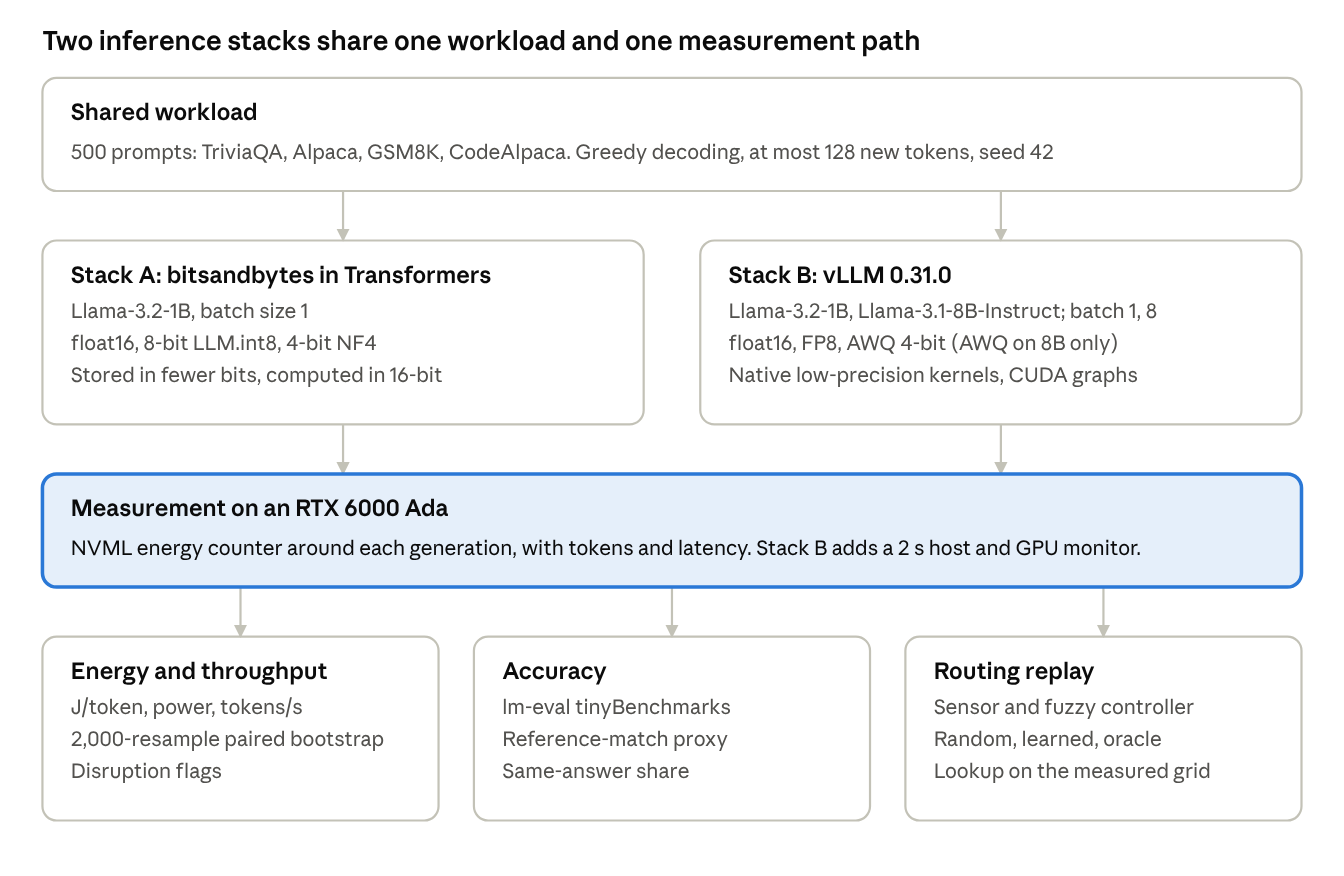
\includegraphics[width=\linewidth]{figs/fig_architecture.png}
\caption[System architecture]{System architecture}
\end{figure}

\section{Experimental workflow}
Every configuration goes through the same steps: warm-up, measurement, logging, then checks. A run enters the analysis only if it passes the disruption check, which we added after finding the pitfall described in section 5.5.

\begin{figure}[htbp]
\centering
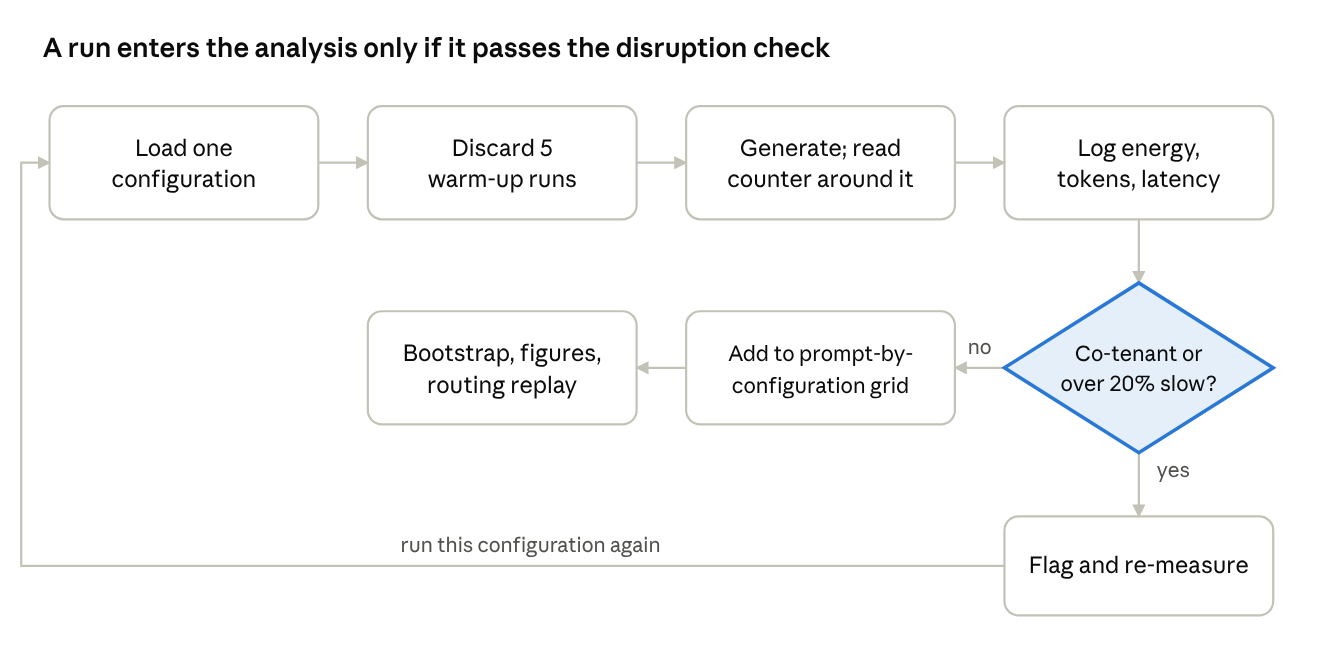
\includegraphics[width=\linewidth]{figs/fig_workflow.png}
\caption[Measurement workflow]{Measurement workflow}
\end{figure}
Stack B applies this check through its monitor and analysis script. Stack A's clean runs had to be identified after the fact from throughput and power, because the check did not yet exist when they were planned.

\section{Modules}

\begingroup\footnotesize\setlength{\tabcolsep}{4pt}
\begin{longtable}{>{\raggedright\arraybackslash}p{32.6mm}>{\raggedright\arraybackslash}p{53.7mm}>{\raggedright\arraybackslash}p{55.3mm}}
\toprule
\textbf{Module} & \textbf{Purpose} & \textbf{Implementation} \\
\midrule
\endhead
Evaluation set builder & Builds 500 unique, stratified prompts; fails rather than pads with duplicates & prepare\_\allowbreak{}eval\_\allowbreak{}dataset.py \\*
Stack A runner & Measures bitsandbytes tiers at batch 1 and computes routing conditions & kaggle\_\allowbreak{}routing\_\allowbreak{}experiment.py \\
Stack B runner & Measures vLLM configurations at batch 1 and 8, with a stall watchdog & vllm\_\allowbreak{}energy\_\allowbreak{}benchmark.py, session5\_\allowbreak{}vllm.sh \\
Energy meter & Reads the GPU's cumulative counter around each generation call & GpuEnergyMeter class (Stack A); Meter class (Stack B) \\
Host monitor & Samples GPU, co-tenant, load and CPU clock data every 2 s (Stack B) & Monitor thread in vllm\_\allowbreak{}energy\_\allowbreak{}benchmark.py \\
Complexity sensor & Computes five normalized prompt features & router/complexity\_\allowbreak{}scorer.py \\
Fuzzy controller & Maps features to a complexity score and a tier & router/fuzzy\_\allowbreak{}controller.py, routellm\_\allowbreak{}bridge.py \\
LoRA adapters & Tier adapters tested for accuracy recovery on Stack A & adapters/, adapter-training.ipynb \\*
Accuracy evaluation & Runs standard benchmarks per configuration & kaggle\_\allowbreak{}accuracy\_\allowbreak{}eval.py, session5\_\allowbreak{}accuracy.sh \\*
Analysis & Bootstrap intervals, routing replay, figures & paper\_\allowbreak{}a\_\allowbreak{}analysis.py, session5\_\allowbreak{}analysis.py, session5\_\allowbreak{}router\_\allowbreak{}replay.py \\*
\bottomrule\noalign{\nobreak}
\end{longtable}
\addtocounter{table}{-1}
\endgroup

Despite its name, routellm\_\allowbreak{}bridge.py is a documented threshold pass-through. It does not load or call a RouteLLM model, because RouteLLM's checkpoints are trained on battles between named models and carry no signal for precision tiers.

\section{Energy measurement}
Energy for a generation call is the change in the GPU's cumulative hardware counter across that call, where $C$ is the NVML reading~\cite{b43} in joules.

\begin{equation}
E_i = C(t_{\mathrm{end}}) - C(t_{\mathrm{start}})
\end{equation}
Throughput and mean power, derived from the same logs, form the basis of the disruption check.

\begin{equation}
T_i = \frac{n_i}{t_i} \qquad\qquad P_i = \frac{E_i}{t_i}
\end{equation}
The two stacks report energy per token differently. Stack A logs each prompt separately, so we take a median over prompts with at least 16 generated tokens. All zero readings came from generations of at most 2 tokens and under 80 ms. The 16-token minimum is a conservative margin: when we varied it from 1 to 64, using non-zero readings, the 4-bit/float16 ratio moved by at most 0.016 within a run and the 8-bit ratio by at most 0.029. Stack B divides total energy by total output tokens, which short generations cannot distort.

\begin{equation}
\text{Stack A: } e = \operatorname{median}_{i:\, n_i \geq 16} \frac{E_i}{n_i}\qquad\qquad \text{Stack B: } e = \frac{\sum_i E_i}{\sum_i n_i}
\end{equation}
In a batched call we attribute energy to prompts in proportion to their output tokens. This is an approximation, since prompts in a batch share one reading, but it does not affect the reported J/token, which uses batch totals, and routing replay uses batch 1.

\begin{equation}
E_i = E_b \cdot \frac{n_i}{\sum_{j \in b} n_j}
\end{equation}
We report each saving against the same model's float16 at the same batch size. Its interval comes from a paired bootstrap over prompts with 2,000 resamples, recomputing the ratio on each resample.

\begin{equation}
\text{saving} = 1 - \frac{e_{\mathrm{config}}}{e_{\mathrm{float16}}}
\end{equation}
\textbf{Algorithm 1: measure one configuration}

\begin{enumerate}
\item Load the configuration, so that it is the only one resident in GPU memory, and record the GPU UUID and driver.
\item Run 5 warm-up generations and discard them.
\item For each prompt or batch, read the counter, generate with greedy decoding up to 128 new tokens, wait for the GPU to finish, and read the counter again. Stack A synchronizes explicitly with torch.cuda.synchronize().
\item Log energy, output tokens, latency, response and correctness for each prompt.
\item On Stack B, sample GPU utilization, power, clocks, co-tenant processes, host load and CPU clock every 2 s throughout, and stop a configuration after 900 s with no progress.
\item Compute energy per token, throughput and mean power, and apply the checks in section 3.2.
\end{enumerate}
\section{Complexity sensor}
The sensor converts a prompt into five features in the range 0 to 1. Continuous features are normalized against fixed ranges calibrated on the 500-prompt set.

\begin{equation}
\hat{x} = \min\!\left(1,\ \max\!\left(0,\ \frac{x - x_{\min}}{x_{\max} - x_{\min}}\right)\right)
\end{equation}

\begingroup\footnotesize\setlength{\tabcolsep}{4pt}
\begin{longtable}{>{\raggedright\arraybackslash}p{36.7mm}>{\raggedright\arraybackslash}p{49.4mm}>{\raggedright\arraybackslash}p{18.3mm}>{\raggedright\arraybackslash}p{34.4mm}}
\toprule
\textbf{Feature} & \textbf{Definition} & \textbf{Range} & \textbf{LOW/MEDIUM and MEDIUM/HIGH edges} \\
\midrule
\endhead
Flesch-Kincaid grade & Readability grade from textstat & 0 to 18 & 5.0, 7.7 \\*
Token length & Characters divided by 4, an approximation & 0 to 154 & 0.086, 0.125 (normalized) \\*
Entropy & Character-level Shannon entropy, in bits & 3.3 to 5.0 & 3.98, 4.16 \\*
Syntax depth & Maximum spaCy dependency-tree depth & 2 to 14 & 4, 5 \\*
Code or maths & 1 for code, LaTeX or maths symbols; code-request words; or two or more numbers with a quantity cue & 0 or 1 & Binary \\*
\bottomrule\noalign{\nobreak}
\end{longtable}
\addtocounter{table}{-1}
\endgroup

The grade and entropy are computed as follows, where $w$, $s$ and $y$ count words, sentences and syllables, and $p_c$ is the share of character $c$.

\begin{equation}
\mathrm{FK} = 0.39\,\frac{w}{s} + 11.8\,\frac{y}{w} - 15.59\qquad\qquad H = -\sum_c p_c \log_2 p_c
\end{equation}
The edges are empirical terciles of each feature on the evaluation set, computed by calibrate\_\allowbreak{}breakpoints.py from the feature values alone, although we did use the difficulty labels when choosing the rule features (section 3.6). We tuned the ranges and edges on the same prompts used for evaluation, a limitation we return to in section 5.8.

\section{Fuzzy controller}
The controller is a Mamdani system built with scikit-fuzzy. MEDIUM is a triangle peaking at the midpoint of the two edges, and LOW and HIGH are saturating trapezoidal shoulders, so a term reaches full membership before the end of the range.

The rule base has 15 rules. Nine cover every combination of terms for the two features that separated the difficulty labels best on this set:


\begingroup\footnotesize\setlength{\tabcolsep}{4pt}
\begin{longtable}{>{\raggedright\arraybackslash}p{52.7mm}>{\raggedright\arraybackslash}p{28.5mm}>{\raggedright\arraybackslash}p{29.0mm}>{\raggedright\arraybackslash}p{28.5mm}}
\toprule
\textbf{Flesch-Kincaid \textbackslash{} Syntax depth} & \textbf{Low} & \textbf{Medium} & \textbf{High} \\
\midrule
\endhead
Low & LOW & LOW & MEDIUM \\*
Medium & MEDIUM & MEDIUM & HIGH \\*
High & MEDIUM & HIGH & HIGH \\*
\bottomrule\noalign{\nobreak}
\end{longtable}
\addtocounter{table}{-1}
\endgroup

Six modifier rules add the other features:

\begin{itemize}
\item Code or maths present gives HIGH.
\item Long length with high readability grade gives HIGH.
\item Long length with medium or low grade gives MEDIUM (two rules).
\item High entropy with high grade gives HIGH.
\item Low grade, short length, low depth and no code gives LOW.
\end{itemize}
Rule strengths use minimum for AND and maximum for aggregation. The output $y$ runs from 0 to 100 with three triangular terms, and centroid defuzzification gives the score $y^{*}$ that selects the tier.

\begin{equation}
y^{*} = \frac{\int y\,\mu(y)\,dy}{\int \mu(y)\,dy}
\end{equation}
\begin{equation}
\text{tier} = \text{low if } y^{*} < 33;\quad \text{middle if } 33 \leq y^{*} \leq 66;\quad \text{high if } y^{*} > 66
\end{equation}
\begin{figure}[htbp]
\centering
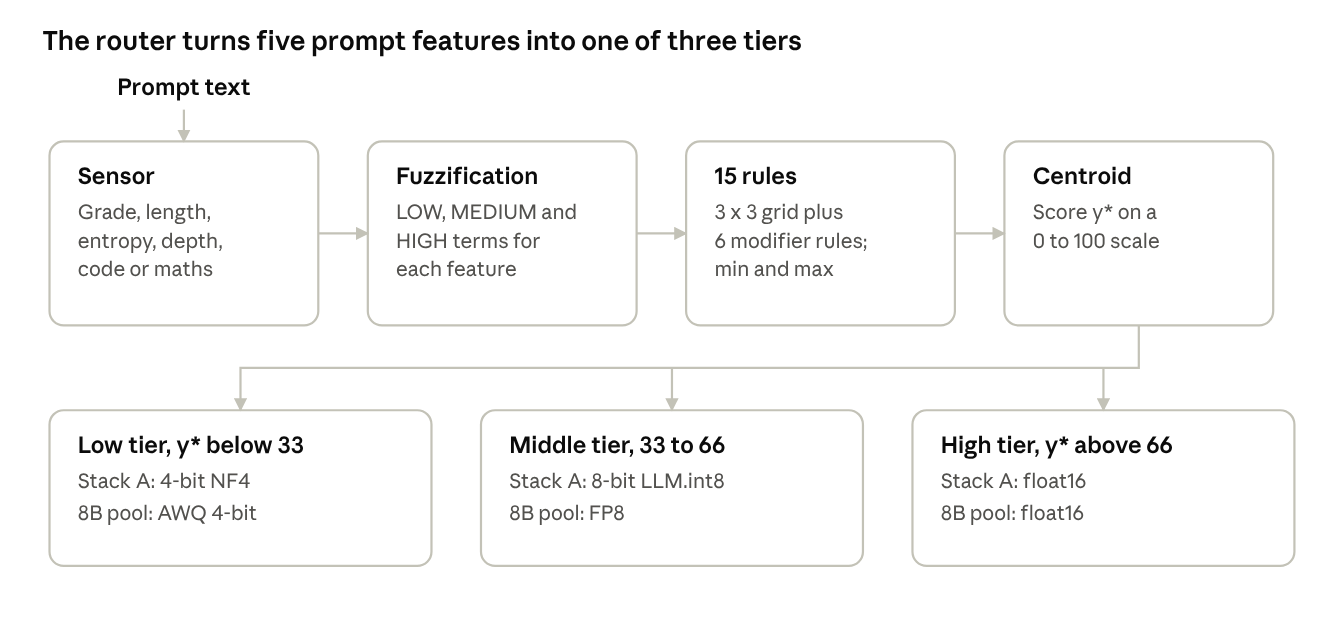
\includegraphics[width=\linewidth]{figs/fig_router.png}
\caption[Router pipeline]{Router pipeline}
\end{figure}
In the two-option 1B/8B pool, the middle and high tiers both map to the larger option.

\textbf{Algorithm 2: route one prompt}

\begin{enumerate}
\item Compute the five raw features of the prompt.
\item Normalize each continuous feature against its fixed range.
\item Fuzzify the features and evaluate all 15 rules.
\item Aggregate the fired output terms and take the centroid $y^{*}$. If no rule fires, set $y^{*} = 50$.
\item Set $w = y^{*}/100$, and return the low tier if $w < 0.33$, the high tier if $w > 0.66$, and the middle tier otherwise.
\end{enumerate}
We reached this design after two rounds of diagnosis. An earlier bridge escalated every score of exactly 50 to 16-bit, and 47\% of prompts scored exactly 50 because no rule discriminated. Fixing both still left 32\% of prompts (161) on the neutral score: 110 from a MEDIUM centroid, and 51 (10.2\%) on which no rule fired and the controller defaulted to 50. Runs 5-7 and all of Session 5 use the corrected router.

\section{LoRA adapters}
We tested three LoRA adapters~\cite{b26} on Stack A to see whether they recover accuracy lost to quantization. They target q\_\allowbreak{}proj and v\_\allowbreak{}proj, with ranks 16, 8 and 4 for the 4-bit, 8-bit and 16-bit tiers, which gives lower precision more capacity. All three were trained on the 4-bit NF4 model, split by a prompt complexity label, so they do not constitute tier-specific quantization-aware training.

\textbf{The adapters are also part of the measured Stack A configurations.} The routing experiment attaches an unmerged adapter to every tier, including float16, in all of runs 1-7; only Session 1 ran without adapters. Stack A energy results therefore describe bitsandbytes with an attached adapter and do not isolate the quantization kernel, a point section 5.1 takes up.

\section{Accuracy and routing evaluation}
We keep two accuracy measures separate. Benchmark accuracy comes from lm-eval-harness on tinyMMLU, tinyHellaswag and tinyGSM8k, with 100 items per task. Routing correctness uses a reference-match proxy on the 500 prompts: numeric match for short numeric answers, normalized substring match for references of up to six words, and stem-level token F1 of at least 0.5 otherwise. Since the proxy is coarse, we interpret only paired differences between policies. tinyGSM8k is reported under flexible-extract scoring, as in the project's logs; strict-match scores are also given in section 5.4, because the choice affects the conclusion.


\begingroup\footnotesize\setlength{\tabcolsep}{4pt}
\begin{longtable}{>{\raggedright\arraybackslash}p{38.3mm}>{\raggedright\arraybackslash}p{59.3mm}>{\raggedright\arraybackslash}p{44.0mm}}
\toprule
\textbf{Policy} & \textbf{Rule} & \textbf{Purpose} \\
\midrule
\endhead
Static & Always one configuration & The baseline a router must outperform \\*
Fuzzy & Algorithm 2 & The system under test \\*
Random-matched & Stack A: exact shuffle of the fuzzy router's tier list, mean of 20 draws. Stack B: random choice with the same mix in expectation, mean of 1,000 draws & Separates routing intelligence from the effect of tier mix \\*
Threshold (Stack A) & The same cuts applied to the plain mean of the five features & Tests what the fuzzy inference adds \\*
Learned (Stack B, 1B/8B pool) & Logistic regression on the same features, predicting whether the cheaper option is correct; 5-fold cross-fitted, thresholds 0.5, 0.7 and 0.9 & Tests one simple learned alternative \\*
Oracle & Stack A: lowest measured energy among correct tiers for that prompt, or lowest overall if none is correct. Stack B: first correct option when ordered by mean energy, or the cheapest on average if none is correct & Indicates the headroom available to routing \\*
\bottomrule\noalign{\nobreak}
\end{longtable}
\addtocounter{table}{-1}
\endgroup

Because the experiment script's own oracle assumed that fewer bits are cheaper, which is false on Stack A, we report the energy-based oracle from the analysis scripts. Only the Stack A form is a per-prompt energy lower bound, which is why the Stack B oracle can cost more than a static tier.

\textbf{Algorithm 3: replay a routing policy}

\begin{enumerate}
\item Build a grid of measured energy and correctness for every prompt and configuration.
\item Score each prompt with the sensor and controller, and map the tiers onto the configurations in the pool.
\item For each policy, select one configuration per prompt and look up its energy and correctness.
\item Report mean energy per request and proxy accuracy, with paired bootstrap intervals against a reference policy.
\end{enumerate}
\section{Statistical analysis}
For energy savings we use a paired bootstrap over prompts, with 2,000 resamples and 95\% percentile intervals, because per-prompt energy need not be normally distributed. Policy comparisons use the same procedure on per-prompt differences. These intervals cover prompt sampling only, not differences in GPU unit, driver or time of day. At batch 8, resampling batches instead of prompts widens them slightly (for example 1B FP8 in run 2, from 36.3--38.6\% to 34.3--40.4\%) without changing the conclusion.

We also computed three further analyses offline from the existing logs, using training/scripts/thesis\_\allowbreak{}extra\_\allowbreak{}analysis.py. They use the same data and involve no new GPU measurement.

\begin{enumerate}
\item \textbf{Accuracy by source dataset.} Paired differences against float16 on each source dataset of the 500 prompts, to check benchmark findings on separate items.
\item \textbf{Threshold sensitivity.} Replay of the fuzzy score at cuts of 25/75, 30/70, 33/66, 40/60 and 45/55, compared with 1,000 random permutations of each resulting tier assignment.
\item \textbf{Feature signal.} Spearman correlation of each feature with correctness and with sensitivity to quantization, where a prompt is sensitive if float16 is correct and the low-precision tier is not. A logistic regression on all five features gives a 5-fold cross-validated AUC.
\end{enumerate}

\section{Reasons for the chosen methodology}

\begingroup\footnotesize\setlength{\tabcolsep}{4pt}
\begin{longtable}{>{\raggedright\arraybackslash}p{38.8mm}>{\raggedright\arraybackslash}p{51.5mm}>{\raggedright\arraybackslash}p{51.3mm}}
\toprule
\textbf{Decision} & \textbf{Reason} & \textbf{Alternative considered} \\
\midrule
\endhead
Hardware energy counter & Measures the GPU directly, without a sampling assumption in the project's own code & Software estimators with coarse sampling, which suit long jobs better than single prompts \\*
One configuration resident at a time & Avoids memory and cache effects from other tiers & Interleaved tiers, tested in run 2, which distribute drift across tiers but were measured under load \\*
Two stacks on one model & Tests whether the outcome depends on implementation & Varying bit-width alone, which hides the implementation effect \\*
vLLM added after Stack A & The research plan named low-bit kernels as the response if bitsandbytes showed no saving & Reframing as a latency study only \\*
Fuzzy controller & Rules are readable and editable; routing added about 10 ms per prompt on the CPU & A learned router alone, retained instead as a baseline \\*
\bottomrule\noalign{\nobreak}
\end{longtable}
\addtocounter{table}{-1}
\endgroup


\chapter{Experimental Setup and System Configuration}
All reported energy runs used NVIDIA RTX 6000 Ada GPUs on one shared SLURM node at Sardar Patel Institute of Technology, with the same 500 prompts, greedy decoding and seed 42. In this chapter, ``not documented'' means that the repository records the value but not the reason for it, and ``not recorded'' means that the value itself is absent.

\section{Hardware}

\begingroup\footnotesize\setlength{\tabcolsep}{4pt}
\begin{longtable}{>{\raggedright\arraybackslash}p{25.2mm}>{\raggedright\arraybackslash}p{39.8mm}>{\raggedright\arraybackslash}p{43.7mm}>{\raggedright\arraybackslash}p{30.1mm}}
\toprule
\textbf{Component} & \textbf{Specification} & \textbf{Reason and contribution} & \textbf{Evidence} \\
\midrule
\endhead
GPU & NVIDIA RTX 6000 Ada Generation, 49,140 MiB, 300 W cap & The college cluster replaced Kaggle after a Kaggle session hung until its 12-hour limit. The GPU exposes the NVML energy counter, and vLLM lists FP8 support on Ada~\cite{b45}. & nvidia-smi logs; NEW.md \\
GPU units & Two on the node: GPU-c53791fb (bus 01:00) and GPU-da9c4cd1 (bus 61:00) & Assigned by the scheduler, not chosen. Recorded because the unit is confounded with time of day (section 5.5). & Run info files \\
CPU & 2 x AMD EPYC 9554, reported as 56 cores per socket, 2 threads per core, 224 logical CPUs & Part of the shared node. Its load is relevant to the host-side slowdown. & lm-eval environment record \\
Memory & 250 GB RAM & Part of the shared node. & CLUSTER\_\allowbreak{}MANUAL.md \\
Job allocation & 1 GPU, 8 CPUs; 32 GB (Stack A), 64 GB (Stack B) & Values not documented, beyond limiting thread pools to the granted CPUs. & sbatch scripts \\
Adapter training & Kaggle, Tesla T4 & The platform available when the adapters were trained. & Notebook output \\
\bottomrule
\end{longtable}
\endgroup

\section{Software}

\begingroup\footnotesize\setlength{\tabcolsep}{4pt}
\begin{longtable}{>{\raggedright\arraybackslash}p{33.3mm}>{\raggedright\arraybackslash}p{33.1mm}>{\raggedright\arraybackslash}p{30.7mm}>{\raggedright\arraybackslash}p{41.7mm}}
\toprule
\textbf{Software} & \textbf{Stack A} & \textbf{Stack B} & \textbf{Reason and contribution} \\
\midrule
\endhead
Operating system & Rocky Linux 9.8 (same node) & Rocky Linux 9.8 & Cluster default \\
NVIDIA driver & 610.43.02 & 610.57.04 & Cluster-managed; the change between stacks is a stated limitation \\
PyTorch, CUDA & 2.13.0+cu130, CUDA 13.0 & 2.13.0+cu130, CUDA 13.0 & Execution framework for both stacks \\
Python & 3.11 & 3.11.14 & Virtual environments built with uv \\
Transformers & Not recorded & 5.17.0 & Stack A uses it as the common drop-in inference path \\
bitsandbytes & Not recorded & Not used for the tiers & Provides the NF4 and LLM.int8() paths under test \\
vLLM & Not used & 0.31.0, CUDA graphs on & Native FP8 and Marlin AWQ kernels, used to test whether the Stack A result depends on implementation \\
lm-eval-harness & 0.4.13 & 0.4.13 & Community-standard, versioned benchmarks \\
PEFT & 0.19.1, recorded by the adapters & Not used & Loads LoRA adapters \\
NVML bindings & pynvml, version not recorded & nvidia-ml-py, version not recorded & Reads the energy counter directly \\
Router libraries & scikit-fuzzy, textstat, spaCy en\_\allowbreak{}core\_\allowbreak{}web\_\allowbreak{}sm; versions not recorded & Same modules, replayed offline & Mamdani inference, readability grade and dependency depth \\
Analysis libraries & pandas, NumPy, SciPy, scikit-learn, Matplotlib; cluster versions not recorded & Same & Bootstrap, replay, correlation and figures \\
\bottomrule
\end{longtable}
\endgroup

Versions marked ``not recorded'' were not captured at the time of the runs. The file requirements.txt predates these runs and does not describe them.

\section{Models and configurations}

\begingroup\footnotesize\setlength{\tabcolsep}{4pt}
\begin{longtable}{>{\raggedright\arraybackslash}p{27.5mm}>{\raggedright\arraybackslash}p{33.4mm}>{\raggedright\arraybackslash}p{27.1mm}>{\raggedright\arraybackslash}p{17.3mm}>{\raggedright\arraybackslash}p{30.7mm}}
\toprule
\textbf{Configuration} & \textbf{Model} & \textbf{Quantization} & \textbf{Adapter} & \textbf{Reason} \\
\midrule
\endhead
Stack A float16 & Llama-3.2-1B~\cite{b36} & None & r=4 attached & Reference tier. The model matches the adapters and fit the earlier T4 target. \\
Stack A 8-bit & Llama-3.2-1B & LLM.int8() & r=8 attached & Common drop-in 8-bit path; computes in 16-bit~\cite{b6} \\
Stack A 4-bit & Llama-3.2-1B & NF4, double quantization, float16 compute & r=16 attached & Common drop-in 4-bit path. Double quantization: not documented. \\
Stack B 1B float16 & Llama-3.2-1B & None & None & Continuity with Stack A \\
Stack B 1B FP8 & Llama-3.2-1B & fp8 & None & Native FP8 on the same model \\
Stack B 8B float16 & Llama-3.1-8B-Instruct~\cite{b36} & None & None & A larger model, expected to be more memory-bound in decoding \\
Stack B 8B FP8 & Llama-3.1-8B-Instruct & fp8 & None & Same comparison at 8B \\
Stack B 8B AWQ & hugging-quants/Meta-Llama-3.1-8B-Instruct-AWQ-INT4 & AWQ, resolved as auto\_\allowbreak{}awq & None & Public 4-bit checkpoint with Marlin kernels \\
\bottomrule
\end{longtable}
\endgroup

The 1B model is a base model and the 8B model is instruction-tuned, so 1B versus 8B accuracy is not a pure comparison of size. No 1B AWQ configuration was run.

\section{Experimental parameters}

\begingroup\footnotesize\setlength{\tabcolsep}{4pt}
\begin{longtable}{>{\raggedright\arraybackslash}p{32.8mm}>{\raggedright\arraybackslash}p{50.3mm}>{\raggedright\arraybackslash}p{58.6mm}}
\toprule
\textbf{Parameter} & \textbf{Value} & \textbf{Reason and contribution} \\
\midrule
\endhead
Decoding & Greedy (do\_\allowbreak{}sample false; temperature 0) & Determinism allows one grid to serve all policies \\
Maximum new tokens & 128 & Fixed cap across configurations; the value is not documented \\
Warm-up & 5 discarded generations & Excludes start-up effects; the count is not documented \\
Batch size & 1 (Stack A); 1 and 8, static batches of consecutive prompts (Stack B) & Batch 1 represents single-request decoding; batch 8 tests whether savings persist \\
Minimum tokens for Stack A J/token & 16 & Excludes generations too short for the counter to advance \\
Seed & 42 & Reproducibility \\
Stack B engine & dtype float16, gpu\_\allowbreak{}memory\_\allowbreak{}utilization 0.85, max\_\allowbreak{}model\_\allowbreak{}len 1024 (energy), 2048 (accuracy) & Values not documented \\
Monitor interval & 2 s & Continuous sampling replaces the failed end-of-run snapshot; the interval is not documented \\
Watchdog & 900 s with no progress & Added after one configuration hung while loading \\
Disruption flag & Any co-tenant, or throughput over 20\% below the configuration's median across runs & Targets the observed signature; the 20\% value is a judgement, not derived \\
Stack A thread pools & OMP, MKL, OpenBLAS and NumExpr limited to 8 & Prevents oversubscription against the granted CPUs \\
Tier cuts & 33 and 66 on a 0 to 100 score & Equal division of the scale; tested in section 5.6 \\
Bootstrap & 2,000 resamples & Interval estimation without a normality assumption \\
\bottomrule
\end{longtable}
\endgroup


\begingroup\footnotesize\setlength{\tabcolsep}{4pt}
\begin{longtable}{>{\raggedright\arraybackslash}p{44.7mm}>{\raggedright\arraybackslash}p{53.0mm}>{\raggedright\arraybackslash}p{43.9mm}}
\toprule
\textbf{LoRA hyperparameter} & \textbf{Value} & \textbf{Reason} \\
\midrule
\endhead
Rank, alpha & 16/32 (4-bit tier), 8/16 (8-bit tier), 4/8 (16-bit tier) & Lower precision receives more capacity; constant alpha/r of 2 \\
Target modules & q\_\allowbreak{}proj, v\_\allowbreak{}proj & Not documented \\
Dropout & 0.05 & Not documented \\
Training data & Up to 2,000 samples per complexity class, maximum length 256 & Not documented \\
Training & 1 epoch, batch size 4, learning rate 2e-4, paged\_\allowbreak{}adamw\_\allowbreak{}8bit, seed 42 & Not documented \\
\bottomrule
\end{longtable}
\endgroup

\section{Datasets}
The evaluation set has 500 unique prompts, built by prepare\_\allowbreak{}eval\_\allowbreak{}dataset.py with seed 42. The builder fails rather than pads with duplicates, because an earlier set contained only 30 unique prompts among 50 rows. Difficulty labels record the source dataset and do not measure difficulty for a given model. The 200/150/150 split is not otherwise justified in the repository.


\begingroup\footnotesize\setlength{\tabcolsep}{4pt}
\begin{longtable}{>{\raggedright\arraybackslash}p{16.8mm}>{\raggedright\arraybackslash}p{17.7mm}>{\raggedright\arraybackslash}p{41.5mm}>{\raggedright\arraybackslash}p{28.1mm}>{\raggedright\arraybackslash}p{31.8mm}}
\toprule
\textbf{Label} & \textbf{Prompts} & \textbf{Source} & \textbf{Reference answer} & \textbf{Reason} \\
\midrule
\endhead
Easy & 200 & TriviaQA, rc.nocontext, validation~\cite{b38} & Short factual answer & Unambiguous answers \\
Medium & 150 & Alpaca, instructions with no input~\cite{b42} & Reference output & Explanation and description tasks \\
Hard & 75 & GSM8K, test split~\cite{b39} & Final numeric answer & Multi-step arithmetic \\
Hard & 75 & CodeAlpaca-20k~\cite{b46} & Reference output & Coding tasks \\
\bottomrule
\end{longtable}
\endgroup

Benchmark accuracy uses tinyBenchmarks~\cite{b37}, with 100 curated items each from MMLU~\cite{b40}, HellaSwag~\cite{b41} and GSM8K~\cite{b39}, selected to reduce GPU time. Scores are IRT-estimated, and lm-eval reports no standard error for them. The adapter training data, combined\_\allowbreak{}cleaned.csv, is not included in the repository.

\section{Experimental runs}
Times are IST start times.


\begingroup\footnotesize\setlength{\tabcolsep}{4pt}
\begin{longtable}{>{\raggedright\arraybackslash}p{28.6mm}>{\raggedright\arraybackslash}p{14.7mm}>{\raggedright\arraybackslash}p{19.8mm}>{\raggedright\arraybackslash}p{22.1mm}>{\raggedright\arraybackslash}p{19.2mm}>{\raggedright\arraybackslash}p{28.7mm}}
\toprule
\textbf{Session} & \textbf{Job} & \textbf{Date and time} & \textbf{GPU unit} & \textbf{Adapters} & \textbf{Use in this thesis} \\
\midrule
\endhead
1, energy & Not in log & 4 Sep 2026 & Not recorded & No & Pitfall evidence; 16-bit value withdrawn \\
4, run 1 & 1505 & 5 Sep & c53791fb & Yes & Before router fix; contended \\
4, run 2, interleaved & 1507 & 5 Sep & c53791fb & Yes & Before router fix; contended \\
4, run 3 & 1529 & 9 Sep & c53791fb & Yes & Contended; not used for results \\
4, run 4 & 1691 & 29 Sep, 11:48 & c53791fb & Yes & 16-bit phase disrupted \\
4, run 5 & 1692 & 30 Sep, 00:05 & da9c4cd1 & Yes & Clean \\
Diagnostic, day & 1706 & 30 Sep, 13:50 & Not recorded & No & Host-side evidence \\
4, run 6 & 1707 & 1 Oct, 00:58 & da9c4cd1 & Yes & Clean \\
Diagnostic, night & 1732 & 3 Oct, 00:55 & Not recorded & No & Host-side evidence \\
4, run 7 & 1733 & 3 Oct, 00:57 & da9c4cd1 & Yes & Clean \\
2, Stack A accuracy & 1784 & 7 Oct & Not read & With and without & Accuracy per tier \\
5, 1B and AWQ accuracy & 2062 & 27 Oct & Not read & No & Stack B accuracy \\
5, 8B accuracy & 2067 & 27 Oct & Not read & No & Stack B accuracy \\
5, run 1 & 2066, 2093 & 28 Oct, 11:02; AWQ batch 8 rerun 29 Oct & c53791fb & No & Clean \\
5, run 2 & 2094 & 29 Oct, 14:23 & c53791fb & No & Clean \\
5, run 3 & 2095 & 29 Oct, 15:19 & c53791fb & No & Clean \\
\bottomrule
\end{longtable}
\endgroup

\section{Evaluation metrics}

\begingroup\footnotesize\setlength{\tabcolsep}{4pt}
\begin{longtable}{>{\raggedright\arraybackslash}p{50.8mm}>{\raggedright\arraybackslash}p{26.2mm}>{\raggedright\arraybackslash}p{64.6mm}}
\toprule
\textbf{Metric} & \textbf{Unit} & \textbf{Purpose} \\
\midrule
\endhead
Energy per token & J/token & Main efficiency measure, defined per stack in section 3.4 \\
Energy per request & J/request & Cost of serving a prompt, used for routing \\
Energy per correct answer & J & Combines cost and proxy accuracy; descriptive only \\
Throughput & tokens/s & Explains energy and detects disruption \\
Mean power & W & Separates working from waiting \\
Benchmark accuracy & 0 to 1 & tinyMMLU, tinyHellaswag acc\_\allowbreak{}norm; tinyGSM8k flexible and strict \\
Proxy correctness & 0 to 1 & Reference match on the 500 prompts, for paired comparison only \\
Same-answer share & \% & Share of prompts answered identically to float16 \\
Cross-validated AUC & 0 to 1 & Whether the features predict a target; 0.5 is chance \\
\bottomrule
\end{longtable}
\endgroup

\section{Testing conditions and deviations from plan}
Stack A checked co-tenants with one end-of-run snapshot, and Stack B sampled them continuously. All clean Stack A runs were overnight, and all Stack B runs were in daytime. Energy is GPU-board energy only.


\begingroup\footnotesize\setlength{\tabcolsep}{4pt}
\begin{longtable}{>{\raggedright\arraybackslash}p{49.3mm}>{\raggedright\arraybackslash}p{40.2mm}>{\raggedright\arraybackslash}p{52.1mm}}
\toprule
\textbf{Plan} & \textbf{What happened} & \textbf{Consequence} \\
\midrule
\endhead
Kaggle T4 for all sessions & Moved to the college cluster after a Kaggle hang & Earlier T4 assumptions do not apply \\
Stack B on three nights & All three runs were in daytime on 28-29 October; the reason is not recorded & No night comparison; confound remains \\
Feature ablation study & Not run & Feature importance is inferred from correlations only \\
Tier-preference router trained on Session 4 data & Not built & A simple logistic baseline was used instead \\
FrugalGPT-style cascade & Optional; not built beyond a stub & Excluded from results \\
APGR and CPT routing metrics & Not reported & Random-matched and oracle comparisons used instead \\
\bottomrule
\end{longtable}
\endgroup

\section{Reproducibility}
From the major-project directory, on a cluster with the same SLURM partition:

\begin{enumerate}
\item Build the prompt set: python training/scripts/prepare\_\allowbreak{}eval\_\allowbreak{}dataset.py --num-prompts 500 --seed 42 --output backend/src/green\_\allowbreak{}weight/data/eval\_\allowbreak{}prompts.jsonl.
\item Run Stack A on separate days: sbatch --export=ALL,RUN\_\allowbreak{}ID=\textless{}n\textgreater{} training/scripts/session4\_\allowbreak{}full\_\allowbreak{}run.sh. Copy each run's output files to routing\_\allowbreak{}run\textless{}n\textgreater{}\_\allowbreak{}* in major-project, because the analysis expects those names.
\item Run Stack A accuracy: sbatch training/scripts/session2\_\allowbreak{}accuracy.sh.
\item Set up Stack B with bash training/scripts/setup\_\allowbreak{}vllm\_\allowbreak{}env.sh, pinning vLLM to 0.31.0 because the script installs the latest version. Then run sbatch --export=ALL,RUN\_\allowbreak{}ID=\textless{}n\textgreater{} training/scripts/session5\_\allowbreak{}vllm.sh.
\item Run Stack B accuracy: sbatch training/scripts/session5\_\allowbreak{}accuracy.sh.
\item Analyse Stack A with python training/scripts/paper\_\allowbreak{}a\_\allowbreak{}analysis.py --clean-runs 5 6 7. Analyse Stack B by passing the run directories to session5\_\allowbreak{}analysis.py, and to session5\_\allowbreak{}router\_\allowbreak{}replay.py with --pool 1b\_\allowbreak{}fp16,8b\_\allowbreak{}awq4 --pool 8b\_\allowbreak{}awq4,8b\_\allowbreak{}fp8,8b\_\allowbreak{}fp16 --batch-size 1.
\item Run python training/scripts/thesis\_\allowbreak{}extra\_\allowbreak{}analysis.py.
\end{enumerate}
The scripts source \textasciitilde{}/greenweight\_\allowbreak{}env.sh and \textasciitilde{}/vllm\_\allowbreak{}env.sh, which are not in the repository, and the Llama models are gated. A Hugging Face token must be supplied through the environment and must not be stored in the repository.


\chapter{Results and Discussion}
The table below gives the answer to each research question and the strength of its evidence, which the following sections present in detail.


\begingroup\footnotesize\setlength{\tabcolsep}{4pt}
\begin{longtable}{>{\raggedright\arraybackslash}p{30.9mm}>{\raggedright\arraybackslash}p{38.3mm}>{\raggedright\arraybackslash}p{36.4mm}>{\raggedright\arraybackslash}p{33.2mm}}
\toprule
\textbf{Question} & \textbf{Answer} & \textbf{Key evidence} & \textbf{Strength} \\
\midrule
\endhead
RQ1: Does lower precision save energy per token? & Depends on the implementation: not on bitsandbytes with adapters attached; yes on vLLM & Stack A 4-bit about equal, 8-bit about 1.8-1.9 times float16; Stack B saves 36-38\% (FP8) and 64\% (AWQ) & Strong for Stack B. Provisional for Stack A pending an adapter-free run \\*
RQ2: What accuracy does it cost? & Not resolved for arithmetic; no clear cost elsewhere at 8B & tinyGSM8k falls 7.2 and 14.1 points under flexible scoring and 6.6 and 5.7 under strict scoring; the fall is not reproduced by coarser paired per-prompt data & Weak: 100 items per task and one run \\*
RQ3: Is measurement reliable on a shared node? & Not without monitoring & float16 ranged from 1.59 to 12.97 J/token, and three safeguards accepted it & Strong for the failure; cause not isolated \\*
RQ4: Can complexity routing beat the best static tier? & No, for these features and pools & Fuzzy matches random at all tested cuts; features predict sensitivity at about chance level & Strong for energy; proxy limits accuracy conclusions \\*
\bottomrule\noalign{\nobreak}
\end{longtable}
\addtocounter{table}{-1}
\endgroup

\section{Stack A: bitsandbytes with attached adapters}
With an adapter attached to every tier, 4-bit used about the same energy per token as float16, and 8-bit about 1.8 to 1.9 times as much, in three clean runs that agree closely.


\begingroup\footnotesize\setlength{\tabcolsep}{4pt}
\begin{longtable}{>{\raggedright\arraybackslash}p{32.4mm}>{\raggedright\arraybackslash}p{42.3mm}>{\raggedright\arraybackslash}p{29.6mm}>{\raggedright\arraybackslash}p{34.5mm}}
\caption[Llama-3.2-1B at batch 1, runs 5 / 6 / 7]{Llama-3.2-1B at batch 1, runs 5 / 6 / 7. Medians over prompts with at least 16 generated tokens (371 for 4-bit, 469 for 8-bit, 447 for 16-bit).}\\
\toprule
\textbf{Tier} & \textbf{Throughput (tokens/s)} & \textbf{Mean power (W)} & \textbf{Energy (J/token)} \\
\midrule
\endfirsthead
\toprule
\textbf{Tier} & \textbf{Throughput (tokens/s)} & \textbf{Mean power (W)} & \textbf{Energy (J/token)} \\
\midrule
\endhead
16-bit float16 & 80.7 / 81.8 / 81.5 & 136 / 142 / 130 & 1.69 / 1.73 / 1.59 \\*
8-bit LLM.int8 & 29.0 / 29.4 / 29.6 & 91 / 91 / 90 & 3.12 / 3.10 / 3.06 \\*
4-bit NF4 & 56.4 / 56.5 / 57.4 & 96 / 97 / 96 & 1.71 / 1.71 / 1.66 \\*
\bottomrule\noalign{\nobreak}
\end{longtable}
\endgroup

The difference between 4-bit and float16 changes sign across runs (+1.3\%, -1.5\%, +4.4\%), so we report the two as about equal. On the 367 prompts where every tier gave at least 16 tokens and a non-zero reading, the ratio of total energy per token was 1.007, 0.965 and 1.065. Each run's interval excludes 1.0, but the differences between runs are larger than the prompt-level intervals.

Among the tiers, float16 draws the most power but is also the fastest. The quantized tiers draw less power but run 1.4 times (4-bit) and 2.8 times (8-bit) slower, and the extra time costs more than the lower power saves.

Memory is a separate benefit. Weights occupy 2.47 GB in float16 (measured), and by calculation about 1.5 GB at 8-bit and 1.0 GB at 4-bit, because the tied embedding remains in float16.

\subsection*{Impact of LoRA adapters on energy measurements}
 The clean runs attach an unmerged LoRA adapter to every tier, with the largest rank on 4-bit. The only adapter-free energy data come from Session 1, whose float16 phase was disrupted.


\begingroup\footnotesize\setlength{\tabcolsep}{4pt}
\begin{longtable}{>{\raggedright\arraybackslash}p{34.5mm}>{\raggedright\arraybackslash}p{52.7mm}>{\raggedright\arraybackslash}p{54.3mm}}
\caption[Stack A with and without adapters]{Stack A with and without adapters. Session 1 values are pooled medians from tier\_\allowbreak{}medians.csv. The sessions also differ in date and possibly in GPU unit.}\\
\toprule
\textbf{Tier} & \textbf{Session 1, no adapters: tokens/s, W, J/token} & \textbf{Runs 5-7, adapters attached: tokens/s, W, J/token} \\
\midrule
\endfirsthead
\toprule
\textbf{Tier} & \textbf{Session 1, no adapters: tokens/s, W, J/token} & \textbf{Runs 5-7, adapters attached: tokens/s, W, J/token} \\
\midrule
\endhead
4-bit NF4 & 67.5, 90, 1.34 & 56.4-57.4, 96-97, 1.66-1.71 \\*
8-bit LLM.int8 & 26.9, 81, 3.02 & 29.0-29.6, 90-91, 3.06-3.12 \\*
16-bit float16 & 11.5, 85, 7.38 (disrupted, withdrawn) & 80.7-81.8, 130-142, 1.59-1.73 \\*
\bottomrule\noalign{\nobreak}
\end{longtable}
\endgroup

The adapter-free 4-bit tier is about 20\% faster and about 20\% cheaper per token than the adapted one, which is consistent with adapter overhead but does not prove it. We have no clean adapter-free float16 energy data. The adapter-free diagnostic reached 109.9 tokens/s, but it had no energy meter and used a different harness, so it cannot supply a J/token value. Whether bare bitsandbytes 4-bit matches float16 has therefore not been measured, and closing this gap requires one clean adapter-free run of all three tiers. The direction of the 8-bit result does agree with Poddar et al.~\cite{b6}, who attribute it to 16-bit computation.

\section{Per token versus per request}
Static 4-bit is 17-25\% cheaper per request than float16 even though it is no cheaper per token, because it generates less text.


\begingroup\footnotesize\setlength{\tabcolsep}{4pt}
\begin{longtable}{>{\raggedright\arraybackslash}p{26.3mm}>{\raggedright\arraybackslash}p{25.7mm}>{\raggedright\arraybackslash}p{28.7mm}>{\raggedright\arraybackslash}p{31.0mm}>{\raggedright\arraybackslash}p{24.3mm}}
\caption[Stack A, all 500 prompts]{Stack A, all 500 prompts.}\\
\toprule
\textbf{Tier} & \textbf{Mean tokens per response} & \textbf{Responses of 2 tokens or fewer (of 500)} & \textbf{Energy (J/request, runs 5 / 6 / 7)} & \textbf{Proxy accuracy} \\
\midrule
\endfirsthead
\toprule
\textbf{Tier} & \textbf{Mean tokens per response} & \textbf{Responses of 2 tokens or fewer (of 500)} & \textbf{Energy (J/request, runs 5 / 6 / 7)} & \textbf{Proxy accuracy} \\
\midrule
\endhead
16-bit float16 & 98.5 & 48 & 166 / 174 / 155 & 0.162 \\*
8-bit LLM.int8 & 103.4 & 30 & 323 / 320 / 317 & 0.186 \\*
4-bit NF4 & 76.5 & 122 & 130 / 130 / 129 & 0.110 \\*
\bottomrule\noalign{\nobreak}
\end{longtable}
\endgroup

The 4-bit tier's responses are 22\% shorter on average, it gives 2.5 times as many near-empty answers, and its proxy accuracy is 5.2 points lower. Its lower request energy therefore reflects less output and fewer correct answers, and is not an efficiency gain. Because token and request energy can move separately, as Vellaisamy et al. warn~\cite{b8}, we report both.

\section{Stack B: vLLM tiers save energy per token}
With vLLM, FP8 and AWQ 4-bit save energy at both batch sizes. Across the three runs, J/token agreed within 2\% for every 8B configuration and within 4.1\% for the 1B configurations.


\begingroup\footnotesize\setlength{\tabcolsep}{4pt}
\begin{longtable}{>{\raggedright\arraybackslash}p{14.7mm}>{\raggedright\arraybackslash}p{21.7mm}>{\raggedright\arraybackslash}p{13.4mm}>{\raggedright\arraybackslash}p{17.8mm}>{\raggedright\arraybackslash}p{18.0mm}>{\raggedright\arraybackslash}p{16.7mm}>{\raggedright\arraybackslash}p{28.0mm}}
\caption[Stack B, medians over three runs]{Stack B, medians over three runs. Saving is the median of per-run savings. The interval is the envelope of the three runs' 95\% paired bootstrap intervals.}\\
\toprule
\textbf{Model} & \textbf{Tier} & \textbf{Batch} & \textbf{J/token} & \textbf{Tokens/s} & \textbf{Mean power (W)} & \textbf{Saving vs float16 [95\% CI]} \\
\midrule
\endfirsthead
\toprule
\textbf{Model} & \textbf{Tier} & \textbf{Batch} & \textbf{J/token} & \textbf{Tokens/s} & \textbf{Mean power (W)} & \textbf{Saving vs float16 [95\% CI]} \\
\midrule
\endhead
1B & float16 & 1 & 0.945 & 307 & 290 & Baseline \\*
1B & FP8 & 1 & 0.604 & 413 & 249 & 36\% [34, 39] \\
8B & float16 & 1 & 5.311 & 56 & 298 & Baseline \\
8B & FP8 & 1 & 3.299 & 87 & 287 & 38\% [38, 38] \\
8B & AWQ 4-bit & 1 & 1.887 & 158 & 298 & 64\% [64, 65] \\
1B & float16 & 8 & 0.139 & 1989 & 275 & Baseline \\
1B & FP8 & 8 & 0.087 & 2743 & 238 & 37\% [36, 39] \\
8B & float16 & 8 & 0.679 & 435 & 296 & Baseline \\*
8B & FP8 & 8 & 0.423 & 673 & 285 & 38\% [37, 38] \\*
8B & AWQ 4-bit & 8 & 0.245 & 1196 & 292 & 64\% [64, 65] \\*
\bottomrule\noalign{\nobreak}
\end{longtable}
\endgroup

\begin{figure}[htbp]
\centering
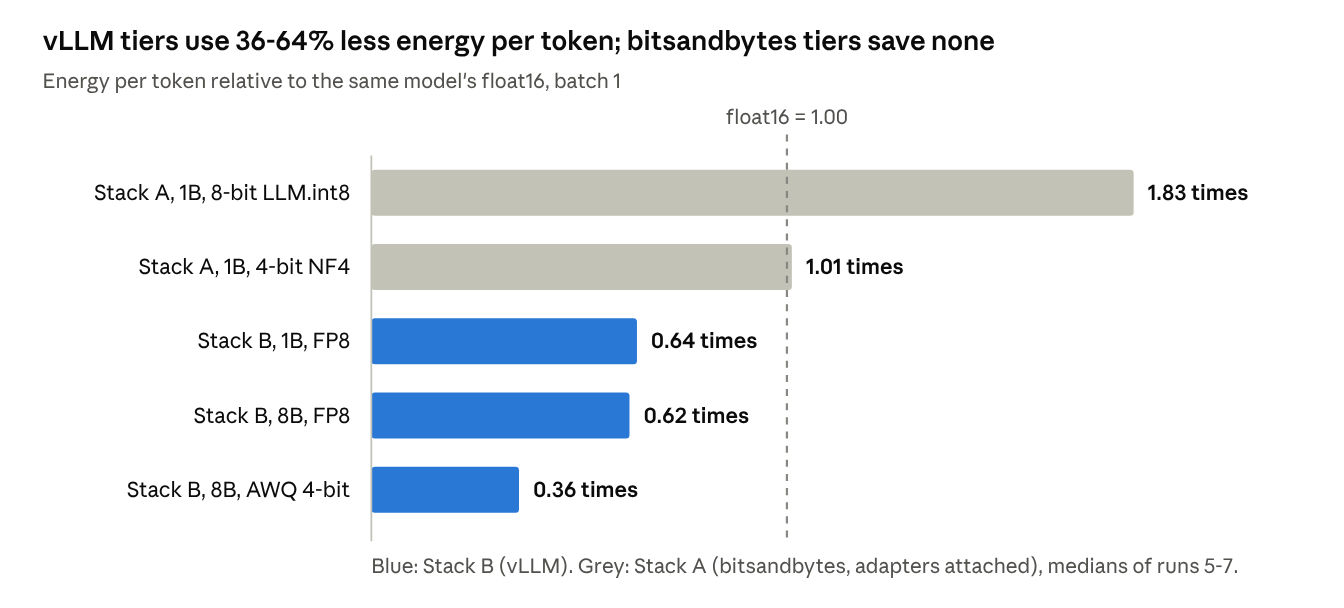
\includegraphics[width=\linewidth]{figs/fig_relative_energy.png}
\caption[Energy per token relative to the same model's float16 at batch 1: vLLM tiers use 36-64\% less, bitsandbytes tiers save none]{Energy per token relative to the same model's float16 at batch 1: vLLM tiers use 36-64\% less, bitsandbytes tiers save none. Source: paper/results.md and paper/analysis/session5\_\allowbreak{}summary.csv; ratios computed from the medians in Tables 5.1 and 5.4.}
\end{figure}
We compare each tier with float16 on its own stack, because the stacks differ in GPU unit, driver, time of day and adapter use. At 8B almost every response reached the 128-token cap on all tiers (mean 127.7 to 127.9 tokens in run 2), so these savings do not come from shorter answers.

\textbf{Why the stacks differ.} Energy is power multiplied by time, and at 8B the power is nearly constant, so the saving comes from time. At batch 1, throughput rises 1.55 times with FP8 and 2.8 times with AWQ, compared with 2 times and 4 times fewer weight bytes. At 1B, FP8 is 1.35 times faster.

\begin{figure}[htbp]
\centering
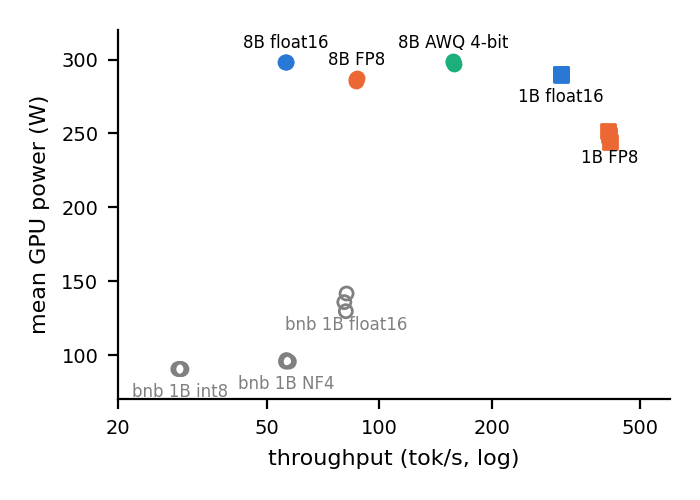
\includegraphics[width=\linewidth]{figs/fig_why.png}
\caption[Throughput and mean power at batch 1]{Throughput and mean power at batch 1.}
\end{figure}
A plausible mechanism is memory traffic: small-batch decoding may be limited by reading weights once per token, and these kernels read fewer bytes and operate on them directly~\cite{b44}. This fits the throughput and power data, but we did not measure memory traffic, so the explanation remains a hypothesis. The design also cannot separate kernel from engine, because vLLM's float16 differs from Stack A's float16 as well.

\textbf{Batch size and stack.} Moving from batch 1 to batch 8 reduces J/token by 6.8 to 7.8 times for every tier, while the relative savings of FP8 and AWQ remain unchanged. vLLM's float16 at 1B is about 41-45\% cheaper per token than Stack A's float16. That comparison crosses GPU units, drivers, times of day and adapter use, and the J/token definitions differ, so it is indicative only.

\textbf{Comparison with prior work.} The following table sets these results beside published figures.


\begingroup\footnotesize\setlength{\tabcolsep}{4pt}
\begin{longtable}{>{\raggedright\arraybackslash}p{36.3mm}>{\raggedright\arraybackslash}p{33.4mm}>{\raggedright\arraybackslash}p{33.1mm}>{\raggedright\arraybackslash}p{36.0mm}}
\caption[Comparison with published results]{Comparison with published results.}\\
\toprule
\textbf{Source} & \textbf{Reported result} & \textbf{This thesis} & \textbf{Assessment} \\
\midrule
\endfirsthead
\toprule
\textbf{Source} & \textbf{Reported result} & \textbf{This thesis} & \textbf{Assessment} \\
\midrule
\endhead
Poddar et al.~\cite{b6} & bitsandbytes almost 2 times at equal batch size & 8-bit about 1.8-1.9 times; 4-bit about 1.0 times with adapters & Agrees for 8-bit. 4-bit is lower, on a different GPU, tools and workload \\*
Basta~\cite{b47} & bitsandbytes int8 saves up to 4 times against FP32 on short generation & 8-bit costs more than float16 in decode-heavy use & Not a direct conflict: FP32 baseline and prefill-heavy case. Not tested here \\*
TokenPowerBench~\cite{b7} & FP8 saves about 30\% at 405B & FP8 saves 36-38\% at 1B and 8B & Same direction; very different scale and hardware \\*
TokenPowerBench~\cite{b7} & vLLM 25-40\% below Transformers & 41-45\% at 1B, float16 & Same direction; the thesis figure is confounded \\*
Vellaisamy et al.~\cite{b8} & Token and request energy can diverge & 4-bit equal per token, cheaper per request & Agrees \\*
\bottomrule\noalign{\nobreak}
\end{longtable}
\endgroup

\section{Accuracy}
We trust the accuracy evidence less than the energy evidence: each benchmark has 100 items and each configuration ran once, so only large differences can be interpreted.


\begingroup\footnotesize\setlength{\tabcolsep}{4pt}
\begin{longtable}{>{\raggedright\arraybackslash}p{14.0mm}>{\raggedright\arraybackslash}p{38.1mm}>{\raggedright\arraybackslash}p{24.3mm}>{\raggedright\arraybackslash}p{33.5mm}>{\raggedright\arraybackslash}p{26.2mm}}
\caption[tinyBenchmarks, 100 items per task, one run per configuration]{tinyBenchmarks, 100 items per task, one run per configuration.}\\
\toprule
\textbf{Stack} & \textbf{Configuration} & \textbf{tinyMMLU} & \textbf{tinyHellaswag} & \textbf{tinyGSM8k} \\
\midrule
\endfirsthead
\toprule
\textbf{Stack} & \textbf{Configuration} & \textbf{tinyMMLU} & \textbf{tinyHellaswag} & \textbf{tinyGSM8k} \\
\midrule
\endhead
A & 1B float16 & 0.433 & 0.636 & 0.062 \\*
A & 1B float16 + adapter & 0.400 & 0.623 & 0.061 \\
A & 1B 8-bit & 0.391 & 0.634 & 0.104 \\
A & 1B 8-bit + adapter & 0.388 & 0.640 & 0.075 \\
A & 1B 4-bit & 0.393 & 0.573 & 0.063 \\
A & 1B 4-bit + adapter & 0.368 & 0.594 & 0.041 \\
B & 1B float16 & 0.433 & 0.629 & 0.092 \\
B & 1B FP8 & 0.380 & 0.624 & 0.084 \\
B & 8B float16 & 0.629 & 0.818 & 0.746 \\*
B & 8B FP8 & 0.640 & 0.823 & 0.674 \\*
B & 8B AWQ 4-bit & 0.663 & 0.802 & 0.605 \\*
\bottomrule\noalign{\nobreak}
\end{longtable}
\endgroup

\begin{figure}[htbp]
\centering
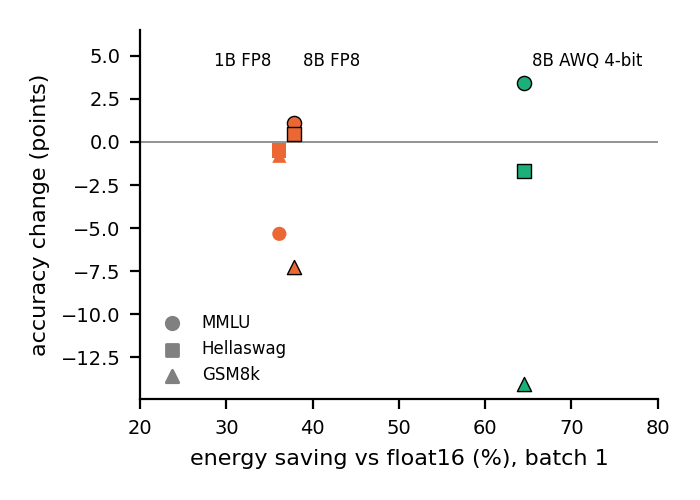
\includegraphics[width=\linewidth]{figs/fig_tradeoff.png}
\caption[Energy saving versus accuracy change]{Energy saving versus accuracy change. Black-edged markers are 8B; plain markers are 1B.}
\end{figure}
At 8B, FP8 and AWQ stay within 3.5 points of float16 on tinyMMLU and tinyHellaswag, in both directions. At 1B, FP8 loses 5.3 points on tinyMMLU and under 1 point on the others. tinyGSM8k scores of 4-10\% are near the floor for this base model, so differences there carry little information.

\textbf{The size of any arithmetic loss is not established.} Under flexible scoring, tinyGSM8k falls by 7.2 points with FP8 and 14.1 points with AWQ. Three checks qualify this.


\begingroup\footnotesize\setlength{\tabcolsep}{4pt}
\begin{longtable}{>{\raggedright\arraybackslash}p{35.5mm}>{\raggedright\arraybackslash}p{20.8mm}>{\raggedright\arraybackslash}p{25.1mm}>{\raggedright\arraybackslash}p{27.1mm}>{\raggedright\arraybackslash}p{27.5mm}}
\caption[tinyGSM8k under two scoring rules, in points]{tinyGSM8k under two scoring rules, in points.}\\
\toprule
\textbf{Configuration} & \textbf{Strict match} & \textbf{Flexible extract} & \textbf{Change from float16: strict} & \textbf{Change from float16: flexible} \\
\midrule
\endfirsthead
\toprule
\textbf{Configuration} & \textbf{Strict match} & \textbf{Flexible extract} & \textbf{Change from float16: strict} & \textbf{Change from float16: flexible} \\
\midrule
\endhead
8B float16 & 0.634 & 0.746 & Baseline & Baseline \\*
8B FP8 & 0.568 & 0.674 & -6.6 & -7.2 \\*
8B AWQ 4-bit & 0.577 & 0.605 & -5.7 & -14.1 \\*
\bottomrule\noalign{\nobreak}
\end{longtable}
\endgroup


\begingroup\footnotesize\setlength{\tabcolsep}{4pt}
\begin{longtable}{>{\raggedright\arraybackslash}p{35.2mm}>{\raggedright\arraybackslash}p{23.9mm}>{\raggedright\arraybackslash}p{39.6mm}>{\raggedright\arraybackslash}p{40.1mm}}
\caption[Paired proxy accuracy at 8B, Stack B run 2, in points]{Paired proxy accuracy at 8B, Stack B run 2, in points. Source: thesis\_\allowbreak{}s5\_\allowbreak{}by\_\allowbreak{}source.csv.}\\
\toprule
\textbf{Source dataset} & \textbf{Prompts} & \textbf{FP8 minus float16 [95\% CI]} & \textbf{AWQ minus float16 [95\% CI]} \\
\midrule
\endfirsthead
\toprule
\textbf{Source dataset} & \textbf{Prompts} & \textbf{FP8 minus float16 [95\% CI]} & \textbf{AWQ minus float16 [95\% CI]} \\
\midrule
\endhead
All & 500 & +0.8 [-1.6, +3.2] & -1.4 [-4.6, +1.6] \\*
TriviaQA & 200 & -1.5 [-6.5, +3.0] & -5.0 [-10.5, 0.0] \\*
Alpaca & 150 & 0.0 [-4.7, +4.0] & +1.3 [-2.7, +5.3] \\*
GSM8K & 75 & +6.7 [0.0, +13.3] & -2.7 [-10.7, +6.7] \\*
CodeAlpaca & 75 & +2.7 [0.0, +6.7] & +4.0 [-2.7, +12.0] \\*
\bottomrule\noalign{\nobreak}
\end{longtable}
\endgroup

\begin{enumerate}
\item \textbf{Sampling noise.} As a rough guide, if the scores are treated as independent proportions on 100 items, the standard error of a difference is about 6.5 points. On that basis FP8's loss is about 1.1 standard errors and AWQ's about 2.2, which passes the usual two-standard-error threshold. This is an approximation, since items are shared and scores are IRT-weighted, and no formal test was possible because per-item outputs were not retained.
\item \textbf{Scoring rule.} AWQ's loss falls from 14.1 to 5.7 points under strict matching (Table 5.7), so much of that gap depends on answer format. FP8's loss barely changes (7.2 to 6.6 points), and both tiers remain below float16 under strict matching.
\item \textbf{Independent items.} On the 75 GSM8K prompts in the evaluation set, FP8 is 6.7 points higher and AWQ's difference includes zero (Table 5.8). This check is limited: the proxy only requires the final number to appear in the output, and responses are capped at 128 tokens.
\end{enumerate}
The evidence therefore allows an arithmetic penalty at AWQ without fixing its size. The paired interval excludes a 14-point loss but includes one of about 6 points, on a coarser measure. On TriviaQA, AWQ's interval of -10.5 to 0.0 points means a smaller factual-recall cost cannot be ruled out either. A full GSM8K evaluation with per-item outputs is needed to resolve the question.

Outputs also change more than scores suggest. Compared with float16, only 18-19\% of answers are identical at 1B FP8, about 7\% at 8B FP8 and 1\% at 8B AWQ. A deployment that needs stable answers should test for this directly.

\textbf{LoRA adapters did not help.} They lower tinyMMLU at every tier and tinyGSM8k at both quantized tiers, with mixed effects on tinyHellaswag. Most differences are a few points and within noise. All three were trained on the 4-bit model (section 3.7), so this does not rule out properly tier-specific training.

\section{A measurement pitfall on a shared node}
The same float16 model consumed between 1.59 and 12.97 J/token across Stack A measurements, while answers and routing decisions stayed the same. Three safeguards accepted the inflated readings.


\begingroup\footnotesize\setlength{\tabcolsep}{4pt}
\begin{longtable}{>{\raggedright\arraybackslash}p{30.3mm}>{\raggedright\arraybackslash}p{23.9mm}>{\raggedright\arraybackslash}p{19.9mm}>{\raggedright\arraybackslash}p{23.5mm}>{\raggedright\arraybackslash}p{15.9mm}>{\raggedright\arraybackslash}p{19.9mm}}
\caption[Stack A float16 across measurements]{Stack A float16 across measurements. Medians over prompts with at least 16 tokens.}\\
\toprule
\textbf{Measurement} & \textbf{GPU unit} & \textbf{Start (IST)} & \textbf{Tokens/s} & \textbf{Mean power (W)} & \textbf{J/token} \\
\midrule
\endfirsthead
\toprule
\textbf{Measurement} & \textbf{GPU unit} & \textbf{Start (IST)} & \textbf{Tokens/s} & \textbf{Mean power (W)} & \textbf{J/token} \\
\midrule
\endhead
Session 1, three runs, no adapters & Not recorded & 4 Sep & 10.5-11.8 & 85 & 7.2-7.8 \\*
Run 4 & c53791fb & 29 Sep, 11:48 & 6.2 & 81 & 12.97 \\*
Run 5 & da9c4cd1 & 30 Sep, 00:05 & 80.7 & 136 & 1.69 \\*
Run 6 & da9c4cd1 & 1 Oct, 00:58 & 81.8 & 142 & 1.73 \\*
Run 7 & da9c4cd1 & 3 Oct, 00:57 & 81.5 & 130 & 1.59 \\*
\bottomrule\noalign{\nobreak}
\end{longtable}
\endgroup

\begin{figure}[htbp]
\centering
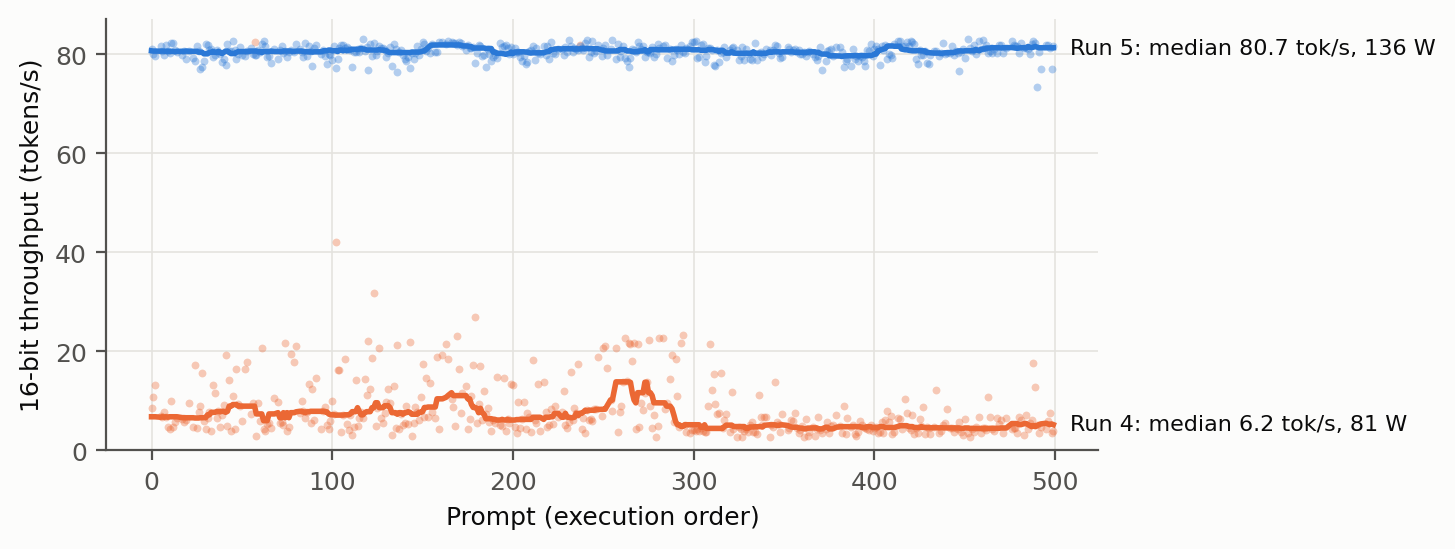
\includegraphics[width=\linewidth]{figs/fig_disruption.png}
\caption[Float16 throughput per prompt in a disrupted run (run 4) and a clean run (run 5)]{Float16 throughput per prompt in a disrupted run (run 4) and a clean run (run 5). Lines are rolling medians over 25 prompts. The two runs used different GPU units.}
\end{figure}
\textbf{Signature of disruption.} Clean float16 runs are fast and power-hungry, whereas disrupted runs are slow and low-power, near the GPU's mostly-idle draw. A waiting GPU still draws substantial power, so energy per token rises roughly with the slowdown.

\textbf{A host-side slowdown.} We ran a diagnostic that timed plain float16 generation with no router, adapters or energy meter. In daytime it ran at a mean of 8.5 tokens/s (range 4.4-25.6), with GPU SM utilization of 0\% at the median and 25\% at the 90th percentile, and CPU time equal to wall time. At night it ran at 109.9 tokens/s with a 1.01 times spread. We interpret this as the GPU waiting on a slowed CPU-side launch path. Because the process stayed on the CPU, the diagnostic alone cannot separate contention from additional work within the software stack, and we did not isolate the mechanism.

Disruption is not specific to 16-bit. In run 2, which interleaved tiers under known load, 16-bit stayed within 1.6\% (as recorded in the experiment log) while 4-bit and 8-bit were inflated 3 to 5 times. In by-tier runs, 16-bit ran last.

\textbf{Why the safeguards missed it.}


\begingroup\footnotesize\setlength{\tabcolsep}{4pt}
\begin{longtable}{>{\raggedright\arraybackslash}p{34.7mm}>{\raggedright\arraybackslash}p{46.5mm}>{\raggedright\arraybackslash}p{60.4mm}}
\toprule
\textbf{Safeguard} & \textbf{What it checks} & \textbf{Why it failed} \\
\midrule
\endhead
End-of-run co-tenant snapshot & Other processes on the GPU, once & Taken at a single moment, and the GPU was not the contended resource. It was empty for run 4 and for runs later confirmed contended. \\*
Repeat-run agreement & Session 1's three runs agreed within 6.6\% & They ran back-to-back under the same conditions. Agreement measured consistency, not cleanliness. Their 16-bit mean of 8.124 J/token is withdrawn; the same 1,500 rows give per-run medians of 7.2 to 7.8 and a pooled median of 7.38. \\*
Automated validator & Completeness, positivity, plausibility, oracle consistency & A uniform slowdown stays inside every limit. The experiment log records that verify\_\allowbreak{}results.py passed run 4. \\*
\bottomrule\noalign{\nobreak}
\end{longtable}
\addtocounter{table}{-1}
\endgroup

\textbf{What the evidence does and does not establish.} Time of day and GPU unit are fully confounded in Stack A: runs 1-4 all used c53791fb and all showed contention or disruption, while clean runs 5-7 all used da9c4cd1, and the diagnostics did not record a UUID. Run 4's 4-bit and 8-bit tiers also drew about 9\% less power than the clean runs at similar throughput, which may reflect a unit or a time effect.

Stack B ran on c53791fb in daytime, at run-median host load of 1.6 to 6, with 100\% median GPU utilization in 29 of 30 configuration-runs and steady throughput. This unit is therefore not simply faulty, although the comparison is not a clean test, because vLLM's CUDA graphs should need far less CPU work per token, and Stack B was not repeated at night or on the other unit.

The evidence supports three claims: float16 readings differed by a factor of about 8 between their extremes, and by 7.7 between run 4 and run 5; three safeguards accepted them; and throughput with power exposed them. It does not support the claim that time of day caused the slowdown. A short diagnostic on each unit, by day and by night, with the UUID recorded, would settle it.

\textbf{Monitoring protocol.} We derived the protocol below from this failure, and Stack B follows it; none of its 30 configuration-runs was flagged. The 20\% throughput rule compares a run with its own configuration's median, so it could miss a slowdown shared by every run: Session 1's float16 runs were all within about 4\% of their median. Continuous GPU utilization is therefore the more independent check.

\begin{enumerate}
\item Report throughput and mean power alongside J/token.
\item Check throughput stability across the run, not only the final mean.
\item Sample GPU utilization, co-tenants, host load and CPU clock continuously, every 2 s.
\item Record the GPU UUID and bus ID for every run, including diagnostics.
\item Flag and re-measure any configuration that departs from its clean baseline by over 20\%.
\item Add a watchdog: one Stack B configuration hung while loading, with the engine at 100\% CPU and the GPU idle.
\end{enumerate}
\section{Routing evaluation}
The fuzzy router did not beat a random router with the same mix on either stack, and it did not beat the best static tier.

\textbf{Stack A.} The table below compares the policies on all 500 prompts.


\begingroup\footnotesize\setlength{\tabcolsep}{4pt}
\begin{longtable}{>{\raggedright\arraybackslash}p{51.3mm}>{\raggedright\arraybackslash}p{38.3mm}>{\raggedright\arraybackslash}p{52.0mm}}
\caption[Stack A routing on 500 prompts]{Stack A routing on 500 prompts. Accuracy is identical across runs because decoding is deterministic.}\\
\toprule
\textbf{Policy} & \textbf{Proxy accuracy} & \textbf{J/request (runs 5 / 6 / 7)} \\
\midrule
\endfirsthead
\toprule
\textbf{Policy} & \textbf{Proxy accuracy} & \textbf{J/request (runs 5 / 6 / 7)} \\
\midrule
\endhead
Static 4-bit & 0.110 & 130 / 130 / 129 \\*
Static 8-bit & 0.186 & 323 / 320 / 317 \\*
Static 16-bit & 0.162 & 166 / 174 / 155 \\*
Fuzzy router & 0.156 & 238 / 239 / 232 \\*
Random, matched mix & 0.166 & 241 / 242 / 234 \\*
Threshold on mean feature & 0.120 & 185 / 184 / 182 \\*
Oracle & 0.258 & 140 / 141 / 134 \\*
\bottomrule\noalign{\nobreak}
\end{longtable}
\endgroup

A paired bootstrap of fuzzy minus static 16-bit gives +71.7 J/request (95\% CI 61.0-82.2), +65.4 (54.9-75.8) and +76.4 (66.5-86.9) in runs 5, 6 and 7. That is 38-49\% more energy, with an accuracy difference of -0.006 (CI -0.034 to +0.020 in runs 5 and 6, and -0.032 to +0.020 in run 7).

In run 5 the sensor sends 61\% of prompts labelled hard to 16-bit against 21\% of those labelled easy. Much of this comes from the code or maths flag, which is set on 73\% of hard prompts and 1\% of easy ones, so it largely recognizes the source dataset; with the flag off, the shares are 37.5\% and 20\%. The router also sends 52\% of all prompts to 8-bit, the most expensive tier. Its choice matches the oracle's on 23.6\% of prompts in run 5, inside the range for a matched random router (mean 25.9\%, 95\% band 22.4 to 29.4). Only 129 of the 500 prompts are answered correctly by any tier under the proxy, which limits what any router can gain.

\textbf{Stack B.} Tiers now differ in cost, so routing has something to save. Two pools were replayed at batch 1.


\begingroup\footnotesize\setlength{\tabcolsep}{4pt}
\begin{longtable}{>{\raggedright\arraybackslash}p{38.6mm}>{\raggedright\arraybackslash}p{26.3mm}>{\raggedright\arraybackslash}p{23.7mm}>{\raggedright\arraybackslash}p{23.2mm}>{\raggedright\arraybackslash}p{24.1mm}}
\caption[Stack B routing replay, run 1]{Stack B routing replay, run 1. Runs 2 and 3 are within 2 J/request, with identical accuracy.}\\
\toprule
\textbf{Policy} & \textbf{8B precision pool: J/request} & \textbf{Accuracy} & \textbf{1B vs 8B AWQ pool: J/request} & \textbf{Accuracy} \\
\midrule
\endfirsthead
\toprule
\textbf{Policy} & \textbf{8B precision pool: J/request} & \textbf{Accuracy} & \textbf{1B vs 8B AWQ pool: J/request} & \textbf{Accuracy} \\
\midrule
\endhead
Static cheapest (8B AWQ; 1B float16) & 240 & 0.350 & 104 & 0.164 \\*
Static 8B FP8 & 422 & 0.372 & Not in pool & Not in pool \\*
Static largest (8B float16; 8B AWQ) & 678 & 0.364 & 240 & 0.350 \\*
Fuzzy router & 477 & 0.368 & 221 & 0.322 \\*
Random, matched mix & 478 & 0.366 & 219 & 0.321 \\*
Learned, cross-fitted & Not run & Not run & 240 & 0.350 \\*
Oracle & 260 & 0.442 & 136 & 0.398 \\*
\bottomrule\noalign{\nobreak}
\end{longtable}
\endgroup

\begin{itemize}
\item \textbf{Precision pool.} Always serving AWQ costs 240 J/request against 678 for float16. Its accuracy gap to FP8 is within noise (-0.022, widest paired CI -0.054 to +0.010). The fuzzy router lands at 477 J, level with random, because it sends a third of prompts to float16 without picking the ones that need it.
\item \textbf{Model-size pool.} The fuzzy router saves 8\% against static 8B AWQ but loses 2.8 points (CI -4.8 to -1.0), again matching random.
\item \textbf{Learned baseline.} A logistic regression on the same five features always chose 8B at thresholds of 0.5 and above. This is a weak test, because the 1B model is correct on only 16.4\% of prompts, so its predicted probability rarely reaches 0.5. The cross-validated AUC of 0.58 in Table 5.13 is the more informative measure.
\item \textbf{Headroom.} In the model-size pool, the oracle would use 43\% less energy than always-8B-AWQ and gain 4.8 points. The oracle knows each outcome in advance and cannot be deployed, so this shows only that routing has headroom in principle. The feature tests below suggest that these surface features are unlikely to capture it.
\end{itemize}
\textbf{Sensitivity to tier cuts.} The negative result does not depend on the choice of 33/66.


\begingroup\footnotesize\setlength{\tabcolsep}{4pt}
\begin{longtable}{>{\raggedright\arraybackslash}p{14.1mm}>{\raggedright\arraybackslash}p{20.9mm}>{\raggedright\arraybackslash}p{19.8mm}>{\raggedright\arraybackslash}p{29.0mm}>{\raggedright\arraybackslash}p{20.1mm}>{\raggedright\arraybackslash}p{29.2mm}}
\caption[Fuzzy score replayed at other cuts, Stack A run 5 and Stack B run 2]{Fuzzy score replayed at other cuts, Stack A run 5 and Stack B run 2. The band is the central 95\% of 1,000 random permutations of the same tier assignment. Reference: static float16 on Stack A, 166 J at 0.162; static AWQ on Stack B, 241 J at 0.350. The 40/60 and 45/55 rows match because no scores fall between those cuts.}\\
\toprule
\textbf{Cuts} & \textbf{Mix, low/mid/high (\%)} & \textbf{Stack A: J/request} & \textbf{Stack A: accuracy [random band]} & \textbf{Stack B 8B: J/request} & \textbf{Stack B 8B: accuracy [random band]} \\
\midrule
\endfirsthead
\toprule
\textbf{Cuts} & \textbf{Mix, low/mid/high (\%)} & \textbf{Stack A: J/request} & \textbf{Stack A: accuracy [random band]} & \textbf{Stack B 8B: J/request} & \textbf{Stack B 8B: accuracy [random band]} \\
\midrule
\endhead
25/75 & 14.4 / 57.6 / 28.0 & 247 & 0.166 [0.152, 0.184] & 467 & 0.368 [0.350, 0.382] \\*
30/70 & 15.6 / 54.8 / 29.6 & 243 & 0.158 [0.150, 0.186] & 469 & 0.368 [0.350, 0.380] \\*
33/66 & 15.6 / 51.6 / 32.8 & 238 & 0.156 [0.148, 0.184] & 477 & 0.368 [0.350, 0.380] \\*
40/60 & 15.8 / 35.2 / 49.0 & 217 & 0.158 [0.146, 0.180] & 519 & 0.362 [0.350, 0.382] \\*
45/55 & 15.8 / 35.2 / 49.0 & 217 & 0.158 [0.146, 0.180] & 519 & 0.362 [0.350, 0.380] \\*
\bottomrule\noalign{\nobreak}
\end{longtable}
\endgroup

At every cut, accuracy falls inside the random band, and no cut reaches the energy of the cheaper reference on either stack. Stack B accuracy at each cut is 1.2 to 1.8 points above static AWQ, at about twice its energy.

These comparisons favour the router, if anything, because its ranges and edges were calibrated on the same 500 prompts.

\textbf{Why the router fails.} We tested the features directly against the outcomes they were intended to predict.


\begingroup\footnotesize\setlength{\tabcolsep}{4pt}
\begin{longtable}{>{\raggedright\arraybackslash}p{31.2mm}>{\raggedright\arraybackslash}p{21.9mm}>{\raggedright\arraybackslash}p{49.9mm}>{\raggedright\arraybackslash}p{35.8mm}}
\caption[Prediction by the five sensor features]{Prediction by the five sensor features. An AUC of 0.5 is chance. Values are from one cross-validation split. Source: thesis\_\allowbreak{}feature\_\allowbreak{}signal.csv.}\\
\toprule
\textbf{Target} & \textbf{Positive prompts} & \textbf{Largest absolute Spearman correlation} & \textbf{Cross-validated AUC} \\
\midrule
\endfirsthead
\toprule
\textbf{Target} & \textbf{Positive prompts} & \textbf{Largest absolute Spearman correlation} & \textbf{Cross-validated AUC} \\
\midrule
\endhead
Stack A: float16 right, 4-bit wrong & 44 & 0.070 (Flesch-Kincaid, p=0.12) & 0.51 \\*
Stack B 8B: float16 right, AWQ wrong & 34 & 0.091 (token length, p=0.042) & 0.43 \\*
Stack A: float16 correct & 81 & 0.070 (code or maths, p=0.12) & 0.52 \\*
Stack B 8B: float16 correct & 182 & 0.184 (code or maths, negative, p\textless{}0.001) & 0.65 \\*
Stack B 1B float16 correct & 82 & 0.122 (code or maths, negative, p=0.006) & 0.58 \\*
\bottomrule\noalign{\nobreak}
\end{longtable}
\endgroup

The two sensitivity targets are what a precision router needs to predict, and both sit at about chance level. The 0.43 is a product of the split: over 20 splits the mean AUC is 0.49 and 0.50, with single-split ranges of 0.43 to 0.53 and 0.45 to 0.54. Bootstrap intervals reach about 0.61, so weak signal is not excluded. The single p=0.042 correlation is one of ten tests on those targets and would not survive a Bonferroni correction.

The features do carry some signal about whether a prompt can be answered at all, mainly through the code or maths indicator, but this does not indicate which tier is sufficient. That distinction fits the router's behaviour: it responds to the difficulty labels and yet does not outperform random assignment. Although the analysis is limited by few positive cases and the proxy metric, the result agrees with GreenServ's ablation, where text complexity did not reduce regret~\cite{b48}, and is consistent with the finer-grained sensitivity reported by DP-LLM~\cite{b50}, although neither study tested this directly.



\section{Discussion}
Our founding assumption did not hold on the Stack A configuration tested: fewer stored bits did not yield less energy per token, because energy depends on execution time and power, not on storage alone. On Stack B, by contrast, savings were large and stable across runs. The following guidance applies within this study's scope:


\begingroup\footnotesize\setlength{\tabcolsep}{4pt}
\begin{longtable}{>{\raggedright\arraybackslash}p{40.2mm}>{\raggedright\arraybackslash}p{40.8mm}>{\raggedright\arraybackslash}p{24.6mm}>{\raggedright\arraybackslash}p{33.3mm}}
\toprule
\textbf{Goal} & \textbf{Guidance from these measurements} & \textbf{Evidence} & \textbf{Confidence} \\
\midrule
\endhead
Reduce energy per token on this GPU class & Use vLLM's FP8 or AWQ tiers & Section 5.3 & High for energy \\*
Reduce memory & bitsandbytes reduces memory; do not assume an energy saving & Section 5.1 & Moderate, pending an adapter-free run \\*
Largest single energy lever & Batch requests where latency permits & 6.8 to 7.8 times, section 5.3 & High \\*
Reasoning-heavy workloads & Evaluate AWQ on the target task first & Section 5.4 & Evidence unresolved \\*
Per-prompt savings & Prefer static AWQ over complexity routing, unless a better predictor is available & Section 5.6 & High for energy; proxy for accuracy \\*
Measuring energy on shared nodes & Log throughput, power and unit identity, continuously & Section 5.5 & High \\*
\bottomrule\noalign{\nobreak}
\end{longtable}
\addtocounter{table}{-1}
\endgroup

A complex prompt need not be sensitive to quantization. Prompt complexity, task difficulty, model uncertainty and quantization sensitivity are separate properties, and this study's five features measure only surface properties of the prompt. The tested router therefore gave no energy benefit over static AWQ, a result that covers these features and this controller, not every complexity-based router. The matched random baseline also shows why comparing a router only with static tiers can mislead.

\section{Limitations and threats to validity}
\begin{itemize}
\item \textbf{Adapters on Stack A.} All clean Stack A energy runs carry attached adapters, so they do not isolate bitsandbytes. This is the most important limitation for RQ1.
\item \textbf{Stack comparison.} The stacks share no quantization scheme, and 4-bit was tested on different models. The only same-model contrast is at 1B, where NF4 is about equal to float16, LLM.int8 costs 1.8 to 1.9 times as much and FP8 saves 36\%. The study compares serving configurations and does not isolate bit-width, engine or kernel.
\item \textbf{Run selection and order.} We identified Stack A's clean runs after the fact from throughput and power, and tier order was fixed in Stack A's by-tier runs.
\item \textbf{Prompt format and token cap.} We sent prompts without a chat template, including to the instruction-tuned 8B model, and most 8B responses reached the 128-token cap, so 8B request energy is largely set by that cap.
\item \textbf{Unit and time confound.} Clean Stack A runs used one unit at night. Stack B used the other unit by day, with a newer driver. Cross-stack comparisons inherit this.
\item \textbf{One GPU model and one node.} Data-centre GPUs and other nodes may differ.
\item \textbf{Counter not independently validated.} We did not check NVML against an external meter. Yang et al. report that nvidia-smi power readings sample only 25\% of runtime on A100 and H100~\cite{b17}, and we did not test whether a similar limit affects the cumulative counter on this GPU. Repeatable readings show consistency, not sensor accuracy.
\item \textbf{GPU-board energy only.} CPU, DRAM, cooling and the router's CPU energy are excluded. Host CPU energy could alter comparisons between stacks.
\item \textbf{Short generations.} On Stack A, 81-89 of 500 4-bit generations, 13-15 of 8-bit and 36-41 of 16-bit read 0 J in the clean runs, all at 2 tokens or fewer. Very short readings can also include catch-up energy from the counter's update steps, hence the 16-token filter.
\item \textbf{Model scope.} Both models are Llama, the 1B is a base model and the 8B is instruction-tuned, and the AWQ checkpoint is a third-party conversion.
\item \textbf{Batching.} We tested static batches of 1 and 8 only, with no continuous batching under live traffic, and left vLLM defaults, including prefix caching, on.
\item \textbf{Accuracy noise.} tinyBenchmarks has 100 items per task, each configuration ran once, no standard error is reported, and per-item outputs were not retained.
\item \textbf{Weak routing metric.} The reference-match proxy is coarse, and credit on numeric prompts can be incidental.
\item \textbf{In-sample calibration.} Router ranges and edges were set on the evaluation prompts, and the rule features were chosen using the same prompts' labels. Difficulty labels reflect the source dataset.
\item \textbf{Controller state.} An independent calculation of the fuzzy rules matched all 500 logged scores, and the logged runs passed each prompt once. A reused controller instance gave different scores on 30 prompts when they were repeated, so long-running use needs a separate check.
\item \textbf{Post hoc analyses.} We performed the analyses in section 3.9 after seeing the main results, so they are exploratory.
\item \textbf{Validator coverage.} verify\_\allowbreak{}results.py does not cover Stack B. Those runs were checked by session5\_\allowbreak{}analysis.py and the monitor. Committed validator output predates runs 4-7, whose verdicts are recorded in the experiment log only.
\end{itemize}

\chapter{Conclusion and Future Work}
Whether fewer bits saved energy depended, in our measurements, on the serving configuration. With bitsandbytes and attached adapters, 4-bit was within about 7\% of float16 per token and 8-bit cost about 1.8 to 1.9 times as much. With vLLM, FP8 and AWQ 4-bit saved 38\% and 64\% per token at 8B, and these savings were stable across runs and batch sizes.

We have not yet established the accuracy cost of these savings. tinyGSM8k fell under both scoring rules, by amounts that depend on the rule, and the fall was not reproduced on separate prompts using a coarser measure.

Measurement validity was a problem in its own right: inflated float16 readings passed three safeguards, and throughput with mean power exposed them. We did not isolate the cause, and time of day remains confounded with GPU unit.

Green-Weight's fuzzy router performed no better than a random router with its tier mix at any tested cut, and on the 8B pool it cost about twice as much energy per request as static AWQ. Its features predicted sensitivity to quantization at about chance level. The oracle shows headroom in principle, but this work does not show that any predictor available before generation can capture it.

\section{Future work}
\begin{enumerate}
\item \textbf{Measure Stack A without adapters.} Run all three tiers in one clean overnight session. This is required to complete RQ1.
\item \textbf{Resolve the unit and time confound.} Run the diagnostic on both GPU units, by day and by night, with the UUID recorded.
\item \textbf{Resolve the accuracy question.} Evaluate full GSM8K at 8B, retaining per-item outputs for paired testing.
\item \textbf{Separate kernel from engine.} Run bitsandbytes and native kernels within one engine where possible, and measure GPU memory bandwidth to test the memory-traffic explanation.
\item \textbf{Widen the scope.} Complete the planned Qwen and batch-32 runs, then test other GPU models and continuous batching.
\item \textbf{Measure whole-system energy.} Add CPU and DRAM energy, and validate NVML with an external meter.
\item \textbf{Test richer routing signals.} Evaluate online or response-level signals, such as bandits~\cite{b48} or self-verification~\cite{b31}, against the same matched baseline, on held-out prompts.
\end{enumerate}

\chapter{Publication}
\section{Manuscript status}
A manuscript based on this work, titled ``Fewer Bits Save Energy Only With the Right Kernels: Measuring Precision and Energy in LLM Inference on a Shared GPU Cluster'', has been prepared. It has not yet been submitted to a journal or conference.

\appendix
\chapter{Number traceability}
The numbers in Chapter 5 trace to files in the repository. Checks added in the final revision (minimum-token sensitivity, repeated AUC splits, batch resampling, oracle agreement and router recalculation) come from training/scripts/thesis\_\allowbreak{}review\_\allowbreak{}checks.py and router\_\allowbreak{}truth\_\allowbreak{}check.py, and are exploratory. Figures derived during thesis preparation are identified as such.


\begingroup\footnotesize\setlength{\tabcolsep}{4pt}
\begin{longtable}{>{\raggedright\arraybackslash}p{35.1mm}>{\raggedright\arraybackslash}p{57.8mm}>{\raggedright\arraybackslash}p{48.7mm}}
\toprule
\textbf{Results in this thesis} & \textbf{Source} & \textbf{Validator or log status} \\
\midrule
\endhead
Table 5.1 and clean rows of Table 5.9 & routing\_\allowbreak{}run\{5,6,7\}\_\allowbreak{}per\_\allowbreak{}prompt.csv; paper/results.md. Recomputed from raw CSVs. & Log: runs 5-6 PASS with 1 WARN; run 7 clean by throughput check. No committed validator output for runs 4-7 \\*
Table 5.2 & paper/analysis/tier\_\allowbreak{}medians.csv; routing\_\allowbreak{}run\{5,6,7\}\_\allowbreak{}per\_\allowbreak{}prompt.csv & Session 1 passed the validator, but its 16-bit value is withdrawn \\
Table 5.3 & routing\_\allowbreak{}run\{5,6,7\}\_\allowbreak{}per\_\allowbreak{}prompt.csv and conditions CSVs. Derived for this thesis. & As Table 5.1 \\
Table 5.4, Figures 5.1 and 5.2 & paper/analysis/session5\_\allowbreak{}summary.csv, session5\_\allowbreak{}paired.csv; results/session5\_\allowbreak{}run\{1,2,3\}\_\allowbreak{}* & verify\_\allowbreak{}results.py does not cover these; session5\_\allowbreak{}analysis.py flagged none \\
Table 5.6, Figure 5.3 & results/session2\_\allowbreak{}j1784; results/session5\_\allowbreak{}acc\_\allowbreak{}j2062, j2067 & No verdict row \\
Tables 5.7, 5.8, 5.12, 5.13 & paper/analysis/thesis\_\allowbreak{}*.csv from training/scripts/thesis\_\allowbreak{}extra\_\allowbreak{}analysis.py. Derived for this thesis; exploratory. & Not validated by verify\_\allowbreak{}results.py \\
Earlier rows of Table 5.9, Figure 5.4 & paper/results.md; routing\_\allowbreak{}run4\_\allowbreak{}per\_\allowbreak{}prompt.csv; results/energy\_\allowbreak{}per\_\allowbreak{}inference.csv & Log: run 4 passed, with its 16-bit phase disrupted \\
GPU units & routing\_\allowbreak{}run\{1-7\}\_\allowbreak{}info.json; run\{4,5,6\}\_\allowbreak{}nvidia\_\allowbreak{}smi.txt. & Not applicable \\
Diagnostics & micro\_\allowbreak{}1706.out, micro\_\allowbreak{}1732.out; results.md & Not applicable \\
Table 5.10 & routing\_\allowbreak{}run\{5,6,7\}\_\allowbreak{}conditions.csv; paper/analysis/routing\_\allowbreak{}run*\_\allowbreak{}conditions\_\allowbreak{}ci.csv, *\_\allowbreak{}paired.csv, *\_\allowbreak{}agreement.csv, *\_\allowbreak{}by\_\allowbreak{}difficulty.csv & Fuzzy-vs-random WARN is reported as a finding \\*
Table 5.11 & paper/analysis/session5\_\allowbreak{}routing\_\allowbreak{}*.csv; results.md & Not covered by verify\_\allowbreak{}results.py \\*
Same-answer share & paper/analysis/session5\_\allowbreak{}paired.csv & Not covered by verify\_\allowbreak{}results.py \\*
\bottomrule\noalign{\nobreak}
\end{longtable}
\endgroup

The figures ``\textasciitilde{}40\% energy savings'' and ``\textless{}1\% accuracy loss'' from early project documents are unverified, came from an assumed linear model, and are not results of this work. The 40- and 64-prompt Qwen and batch-32 trials and the 10-prompt smoke tests are excluded from the results.


\clearpage\phantomsection
\addcontentsline{toc}{chapter}{Bibliography}
\begin{thebibliography}{99}
\bibitem{b1} E. Strubell, A. Ganesh, A. McCallum, ``Energy and Policy Considerations for Deep Learning in NLP,'' ACL 2019. \href{https://arxiv.org/abs/1906.02243}{arXiv:1906.02243}
\bibitem{b2} R. Schwartz, J. Dodge, N. A. Smith, O. Etzioni, ``Green AI,'' 2019. \href{https://arxiv.org/abs/1907.10597}{arXiv:1907.10597}
\bibitem{b3} D. Patterson et al., ``Carbon Emissions and Large Neural Network Training,'' 2021. \href{https://arxiv.org/abs/2104.10350}{arXiv:2104.10350}
\bibitem{b4} A. S. Luccioni, S. Viguier, A.-L. Ligozat, ``Estimating the Carbon Footprint of BLOOM, a 176B Parameter Language Model,'' 2022. \href{https://arxiv.org/abs/2211.02001}{arXiv:2211.02001}
\bibitem{b5} S. Samsi et al., ``From Words to Watts: Benchmarking the Energy Costs of Large Language Model Inference,'' 2023. \href{https://arxiv.org/abs/2310.03003}{arXiv:2310.03003}
\bibitem{b6} S. Poddar, P. Koley, J. Misra, N. Ganguly, S. Ghosh, ``Towards Sustainable NLP: Insights from Benchmarking Inference Energy in Large Language Models,'' NAACL 2025, pp. 12688-12704. \url{https://aclanthology.org/2025.naacl-long.632/}
\bibitem{b7} C. Niu et al., ``TokenPowerBench: Benchmarking the Power Consumption of LLM Inference,'' AAAI 2026. \href{https://arxiv.org/abs/2512.03024}{arXiv:2512.03024}
\bibitem{b8} P. Vellaisamy, V. Lam, S. Blanton, J. P. Shen, ``Characterization of Request and Token Energy Costs for LLM Inference Workloads on GPU Platforms,'' IISWC 2026. \href{https://arxiv.org/abs/2608.28044}{arXiv:2608.28044}
\bibitem{b9} G. Wilkins, S. Keshav, R. Mortier, ``Offline Energy-Optimal LLM Serving: Workload-Based Energy Models for LLM Inference on Heterogeneous Systems,'' HotCarbon 2024. \href{https://arxiv.org/abs/2407.04014}{arXiv:2407.04014}
\bibitem{b10} J. Stojkovic, E. Choukse, C. Zhang, I. Goiri, J. Torrellas, ``Towards Greener LLMs: Bringing Energy-Efficiency to the Forefront of LLM Inference,'' 2024. \href{https://arxiv.org/abs/2403.20306}{arXiv:2403.20306}
\bibitem{b11} J. Stojkovic, C. Zhang, I. Goiri, J. Torrellas, E. Choukse, ``DynamoLLM: Designing LLM Inference Clusters for Performance and Energy Efficiency,'' 2024. \href{https://arxiv.org/abs/2408.00741}{arXiv:2408.00741}
\bibitem{b12} P. Patel et al., ``POLCA: Power Oversubscription in LLM Cloud Providers,'' 2023. \href{https://arxiv.org/abs/2308.12908}{arXiv:2308.12908}
\bibitem{b13} J. You, J.-W. Chung, M. Chowdhury, ``Zeus: Understanding and Optimizing GPU Energy Consumption of DNN Training,'' USENIX NSDI 2023. \url{https://www.usenix.org/conference/nsdi23/presentation/you}
\bibitem{b14} A. Faiz et al., ``LLMCarbon: Modeling the End-to-End Carbon Footprint of Large Language Models,'' ICLR 2024. \href{https://arxiv.org/abs/2309.14393}{arXiv:2309.14393}
\bibitem{b15} P. Henderson et al., ``Towards the Systematic Reporting of the Energy and Carbon Footprints of Machine Learning,'' JMLR, vol. 21, 2020. \href{https://arxiv.org/abs/2002.05651}{arXiv:2002.05651}
\bibitem{b16} L. F. W. Anthony, B. Kanding, R. Selvan, ``Carbontracker: Tracking and Predicting the Carbon Footprint of Training Deep Learning Models,'' ICML Workshop, 2020. \href{https://arxiv.org/abs/2007.03051}{arXiv:2007.03051}
\bibitem{b17} Z. Yang, K. Adamek, W. Armour, ``Part-time Power Measurements: nvidia-smi's Lack of Attention,'' 2023, revised 2024, DOI 10.1109/SC41406.2024.00028. \href{https://arxiv.org/abs/2312.02741}{arXiv:2312.02741}
\bibitem{b18} T. Mytkowicz, A. Diwan, M. Hauswirth, P. F. Sweeney, ``Producing Wrong Data Without Doing Anything Obviously Wrong!,'' ASPLOS 2009, pp. 265-276. \url{https://doi.org/10.1145/1508244.1508275}
\bibitem{b19} T. Hoefler, R. Belli, ``Scientific Benchmarking of Parallel Computing Systems,'' SC 2015. \url{https://doi.org/10.1145/2807591.2807644}
\bibitem{b20} T. Dettmers, M. Lewis, Y. Belkada, L. Zettlemoyer, ``LLM.int8(): 8-bit Matrix Multiplication for Transformers at Scale,'' NeurIPS 2022. \href{https://arxiv.org/abs/2208.07339}{arXiv:2208.07339}
\bibitem{b21} T. Dettmers, A. Pagnoni, A. Holtzman, L. Zettlemoyer, ``QLoRA: Efficient Finetuning of Quantized LLMs,'' 2023. \href{https://arxiv.org/abs/2305.14314}{arXiv:2305.14314}
\bibitem{b22} E. Frantar, S. Ashkboos, T. Hoefler, D. Alistarh, ``GPTQ: Accurate Post-Training Quantization for Generative Pre-trained Transformers,'' ICLR 2023. \href{https://arxiv.org/abs/2210.17323}{arXiv:2210.17323}
\bibitem{b23} J. Lin et al., ``AWQ: Activation-aware Weight Quantization for LLM Compression and Acceleration,'' MLSys 2024. \href{https://arxiv.org/abs/2306.00978}{arXiv:2306.00978}
\bibitem{b24} G. Xiao et al., ``SmoothQuant: Accurate and Efficient Post-Training Quantization for Large Language Models,'' ICML 2023. \href{https://arxiv.org/abs/2211.10438}{arXiv:2211.10438}
\bibitem{b25} Y. Park, J. Hyun, S. Cho, B. Sim, J. W. Lee, ``Any-Precision LLM: Low-Cost Deployment of Multiple, Different-Sized LLMs,'' ICML 2024. \href{https://arxiv.org/abs/2402.10517}{arXiv:2402.10517}
\bibitem{b26} E. J. Hu et al., ``LoRA: Low-Rank Adaptation of Large Language Models,'' 2021. \href{https://arxiv.org/abs/2106.09685}{arXiv:2106.09685}
\bibitem{b27} W. Kwon et al., ``Efficient Memory Management for Large Language Model Serving with PagedAttention,'' SOSP 2023. \href{https://arxiv.org/abs/2309.06180}{arXiv:2309.06180}
\bibitem{b28} L. Chen, M. Zaharia, J. Zou, ``FrugalGPT: How to Use Large Language Models While Reducing Cost and Improving Performance,'' 2023. \href{https://arxiv.org/abs/2305.05176}{arXiv:2305.05176}
\bibitem{b29} I. Ong et al., ``RouteLLM: Learning to Route LLMs with Preference Data,'' 2024. \href{https://arxiv.org/abs/2406.18665}{arXiv:2406.18665}
\bibitem{b30} D. Ding et al., ``Hybrid LLM: Cost-Efficient and Quality-Aware Query Routing,'' ICLR 2024. \href{https://arxiv.org/abs/2404.14618}{arXiv:2404.14618}
\bibitem{b31} P. Aggarwal et al., ``AutoMix: Automatically Mixing Language Models,'' NeurIPS 2024. \href{https://arxiv.org/abs/2310.12963}{arXiv:2310.12963}
\bibitem{b32} Q. J. Hu et al., ``RouterBench: A Benchmark for Multi-LLM Routing System,'' 2024. \href{https://arxiv.org/abs/2403.12031}{arXiv:2403.12031}
\bibitem{b33} L. A. Zadeh, ``Fuzzy Sets,'' Information and Control, vol. 8, no. 3, pp. 338-353, 1965. \url{https://doi.org/10.1016/S0019-9958(65)90241-X}
\bibitem{b34} E. H. Mamdani, S. Assilian, ``An Experiment in Linguistic Synthesis with a Fuzzy Logic Controller,'' Int. J. Man-Machine Studies, vol. 7, no. 1, pp. 1-13, 1975. \url{https://doi.org/10.1016/S0020-7373(75)80002-2}
\bibitem{b35} J. P. Kincaid et al., ``Derivation of New Readability Formulas for Navy Enlisted Personnel,'' Naval Technical Training Command, Research Branch Report 8-75, 1975. \url{https://apps.dtic.mil/sti/pdfs/ADA006655.pdf}
\bibitem{b36} A. Grattafiori et al., ``The Llama 3 Herd of Models,'' 2024. \href{https://arxiv.org/abs/2407.21783}{arXiv:2407.21783}
\bibitem{b37} F. M. Polo et al., ``tinyBenchmarks: Evaluating LLMs with Fewer Examples,'' ICML 2024. \href{https://arxiv.org/abs/2402.14992}{arXiv:2402.14992}
\bibitem{b38} M. Joshi, E. Choi, D. S. Weld, L. Zettlemoyer, ``TriviaQA: A Large Scale Distantly Supervised Challenge Dataset for Reading Comprehension,'' 2017. \href{https://arxiv.org/abs/1705.03551}{arXiv:1705.03551}
\bibitem{b39} K. Cobbe et al., ``Training Verifiers to Solve Math Word Problems,'' 2021. \href{https://arxiv.org/abs/2110.14168}{arXiv:2110.14168}
\bibitem{b40} D. Hendrycks et al., ``Measuring Massive Multitask Language Understanding,'' ICLR 2021. \href{https://arxiv.org/abs/2009.03300}{arXiv:2009.03300}
\bibitem{b41} R. Zellers et al., ``HellaSwag: Can a Machine Really Finish Your Sentence?,'' ACL 2019. \href{https://arxiv.org/abs/1905.07830}{arXiv:1905.07830}
\bibitem{b42} R. Taori et al., ``Stanford Alpaca: An Instruction-following LLaMA Model,'' GitHub, 2023. \url{https://github.com/tatsu-lab/stanford_alpaca}
\bibitem{b43} NVIDIA, ``NVML API Reference.'' \url{https://docs.nvidia.com/deploy/nvml-api/index.html}
\bibitem{b44} E. Frantar et al., ``Marlin,'' IST-DASLab software repository. \url{https://github.com/IST-DASLab/marlin}
\bibitem{b45} vLLM project, ``Quantization,'' documentation. \url{https://docs.vllm.ai/en/latest/features/quantization/}
\bibitem{b46} sahil2801, ``CodeAlpaca-20k,'' Hugging Face dataset. \url{https://huggingface.co/datasets/sahil2801/CodeAlpaca-20k}
\bibitem{b47} P. Basta, ``Towards Green AI: Evaluating Energy Efficiency for Quantized LLM Inference,'' Master's thesis, University of Waterloo, 2026. \href{https://arxiv.org/abs/2610.17531}{arXiv:2610.17531}
\bibitem{b48} T. Ziller, S. Ilager, A. Tundo, E. Bartocci, L. Mariani, I. Brandic, ``GreenServ: Energy-Efficient Context-Aware Dynamic Routing for Multi-Model LLM Inference,'' 2026, under submission. \href{https://arxiv.org/abs/2601.17551}{arXiv:2601.17551}
\bibitem{b49} M. A. R. Siddiqui, D. Rojas, C. Yang, W. Cui, Y. Shi, Y. Chen, ``Measured Joules, Learned Routes: Learning to Route for Energy-Efficient LLM Serving,'' 2026, in submission. \href{https://arxiv.org/abs/2609.23085}{arXiv:2609.23085}
\bibitem{b50} S. Kwon, S. H. Seo, J. W. Lee, Y. Park, ``DP-LLM: Runtime Model Adaptation with Dynamic Layer-wise Precision Assignment,'' NeurIPS 2025. \url{https://proceedings.neurips.cc/paper_files/paper/2025/file/d56b84c063265da949fe0feb815dcce8-Paper-Conference.pdf}
\bibitem{b51} F. Liu et al., ``FlexQuant: A Flexible and Efficient Dynamic Precision Switching Framework for LLM Quantization,'' Findings of EMNLP 2025, pp. 4152-4161. \url{https://aclanthology.org/2025.findings-emnlp.221.pdf}
\bibitem{b52} D. Wang et al., ``MoBiQuant: Mixture-of-Bits Quantization for Token-Adaptive Any-Precision LLM,'' 2026. \href{https://arxiv.org/abs/2602.20191}{arXiv:2602.20191}
\bibitem{b53} Y. Moslem, J. D. Kelleher, ``Dynamic Model Routing and Cascading for Efficient LLM Inference: A Survey,'' 2026. \href{https://arxiv.org/abs/2603.04445}{arXiv:2603.04445}
\end{thebibliography}

\end{document}
